\documentclass{moncours}
\usepackage{float}
\makeindex

\begin{document}

\renewcommand{\labelitemi}{\textbullet}
\renewcommand{\labelitemii}{$\circ$} 

\frontmatter
%couvertureFlo
\titlePage[./images/pageGarde2]{Informatique}{Fiches MITIC Teams}{Institut Florimont}{\textcopyright\ Tout droit réservé. Crédit photographie couverture : Institut Florimont. Illustration des premières pages de chapitre issue de \emph{Codex Leicester} de Leonardo da Vinci (domaine public). \\ Version : octobre 2020} 

% TOC
\pagestyle{empty} % No headers

\tableofcontents % Print the table of contents itself
\cleardoublepage % Forces the first chapter to start on an odd page so it's on the right
\pagestyle{fancy} % Print headers again

%\cleardoublepage % on force une page impaire
%\vspace*{1cm}

\section*{Calendrier des différentes activités (5\up{e})}\index{Calendrier des activités}  

\vfill

\begingroup % permet de bloquer le arraystretch à ce groupe seulement
\renewcommand{\arraystretch}{1.2}
\begin{center}
\begin{tabular}{|l|l|c|l|l|}
\hline
\multirow{2}{*}{\textbf{Nom de la fiche}} & \multirow{2}{*}{\textbf{Matière}} & \multirow{2}{*}{\textbf{Page}} & \textbf{Date de} & \textbf{Nom du} \\
 &  &  & \textbf{réalisation} & \textbf{professeur} \\ \hline
%\rowcolor[gray]{0.8}\multicolumn{5}{|l|}{Rentrée scolaire} \\ \hline 
%\emph{La plateforme Flore} & (Titulaire) & \pageref{plateformeFlore} & & \phantom{xxxxxxxxxxxxxxxx}  \\ \hline
%
% avant les vacances d'octobre
%
\rowcolor[gray]{0.8}\multicolumn{5}{|l|}{Avant les vacances d'octobre} \\ \hline
\emph{Tableur : séance 1} & Physique-Chimie & \pageref{ficheTableur5e1} & & \\ \hline
\emph{Texte : séance 1} & Français & \pageref{ficheTexte5e1} & & \\ \hline \hline
%
% avant les vacances de Noël
%
\rowcolor[gray]{0.8}\multicolumn{5}{|l|}{Avant les vacances de Noël} \\ \hline
\emph{Tableur : séance 2} & Mathématiques & \pageref{ficheTableur5e2} & & \\ \hline

\emph{Scratch : séance 1} & Mathématiques & \pageref{ficheScratch5e1} & & \\ \hline \hline
%
% avant les vacances de février
%
%\rowcolor[gray]{0.8}\multicolumn{5}{|l|}{Avant les vacances de février} \\ \hline
%
% avant les vacances de printemps
%
\rowcolor[gray]{0.8}\multicolumn{5}{|l|}{Avant les vacances de printemps} \\ \hline
\emph{Texte : séance 2} & Anglais & \pageref{ficheTexte5e2} & & \\ \hline
\emph{Scratch : séance 2} & Mathématiques & \pageref{ficheScratch5e2} & & \\ \hline
\emph{Son : séance 1} & Anglais & \pageref{ficheSon5e1} & & \\ \hline \hline
%
% avant les vacances d'été
%
\rowcolor[gray]{0.8}\multicolumn{5}{|l|}{Avant les vacances d'été} \\ \hline
\emph{Image : séance 1} & Français & \pageref{ficheImage5e1} & & \\ \hline
\emph{Scratch : séance 3} & Mathématiques & \pageref{ficheScratch5e3} & & \\ \hline \hline
%
% avant la fin du semestre de cours
%
\rowcolor[gray]{0.8}\multicolumn{5}{|l|}{Avant la fin du semestre de cours (pour les cours au semestre)} \\ \hline
\emph{Tableur : séance 3} & Géographie & \pageref{ficheTableur5e3} & & \\ \hline
\emph{Texte : séance 3} & Histoire & \pageref{ficheTexte5e3} & & \\ \hline
\emph{Image : séance 2} & Arts visuels & \pageref{ficheImage5e2} & & \\ \hline
%\emph{Son : séance 2} & Musique & \pageref{ficheSon5e2} & & \\ \hline
\end{tabular}
\end{center}
\endgroup

\vfill

%\cleardoublepage % on force une page impaire pour le clavier
\section*{Les touches spéciales du clavier}\index{Clavier}\index{Touches spéciales}

\vfill

\begin{center}
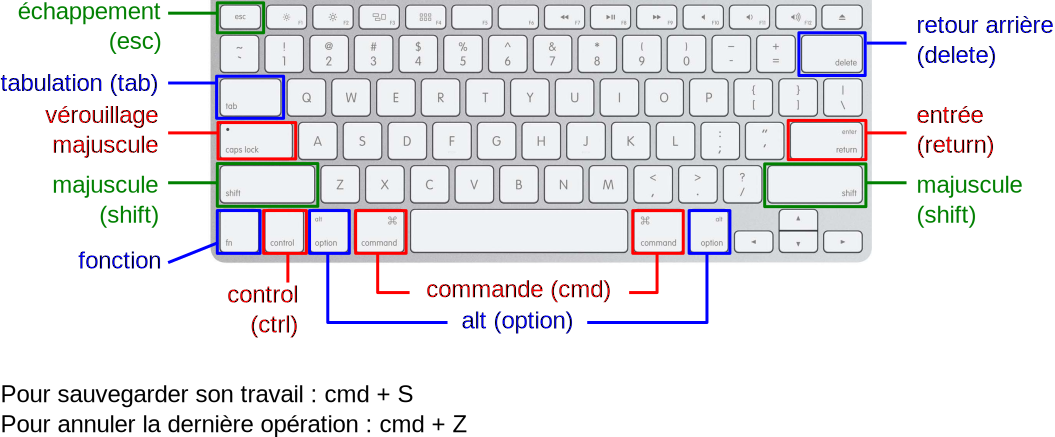
\includegraphics[angle=90,width=.6\textwidth]{./images/generales/clavierTouches}
\end{center}

\vfill

%\cleardoublepage % on force une page impaire pour la philosophie du document
%\chapter*{Philosophie du document}


\prof{\textbf{ceci est la version professeur du document.} L'icône du professeur est suivie par des informations complémentaires qui n'apparaissent pas dans la version élève.}  

Vous avez entre les mains le deuxième tome d'une série de trois fascicules qui accompagneront les élèves des classes de 6\up{e}, 5\up{e} et 4\up{e} jusqu'au moment où ils recevront un ordinateur qu'ils seront en mesure d'exploiter au mieux pour leur travail.

\vspace{18pt}

Ce document se présente sous la forme d'un livret qui rassemble des fiches MITIC\footnote{MITIC : Médias, Images et Technologies de l'Information et de la Communication.} permettant aux élèves d'apprendre à utiliser les logiciels et espaces numériques mis à leur disposition. Pour l'année de 5\up{e}, sont traités les logiciels \emph{Microsoft Word} (traitement de texte), \emph{Microsoft Excel} (tableur grapheur), \emph{Gimp} (retouche d'image), \emph{Audacity} (traitement des fichiers son) et \emph{Scratch} (programmation). Au début de chaque chapitre un lien permettant de télécharger le logiciel est fourni.

\vspace{18pt}


Chaque fiche est conçue pour être exploitée à plusieurs occasions et dans des matières différentes, à chaque fois lors d'une séance de 45 minutes. La fiche sur le tableur, par exemple, est découverte en physique-chimie (\emph{Séance 1}), exploitée à nouveau en mathématiques (\emph{Séance 2}) puis en histoire-géographie (\emph{Séance 3}) selon un calendrier proposé en début de fiche. Nous avons à chaque fois essayé de faire coïncider les notions abordées dans la fiche avec le programme de la matière concernée.

\vspace{18pt}
\prof{
Professeurs, c'est à vous que revient la tâche délicate d'inclure le contenu de ces fiches dans votre progression. À vous de le faire vivre : arriver en salle informatique et demander aux élèves de remettre en forme un texte de Molière ne présente que peu d'intérêt pédagogique. Donnez du sens à ces fiches et profitez-en pour diversifier votre enseignement. N'hésitez pas à exploiter dans vos cours les techniques présentées dans ce fascicule afin que les élèves utilisent plusieurs fois leurs nouvelles compétences et, par là-même, les pérennisent.
}
%\vspace{18pt}

%Ces fiches MITIC sont appelées à évoluer. N'hésitez pas à nous transmettre vos suggestions et nous signaler toute erreur relevée par courriel à l'adresse \texttt{flo-mitic@florimont.ch}.

%\vspace{18pt}

Merci d'avance à tous pour votre implication.

\vspace{18pt}

L'équipe de rédaction.

\vspace{2cm}

% \emph{Remarque : il existe une version professeur de ce document, contenant des informations complémentaires, disponible sur l'ENT de l'école.}

  


% Début des chapitres
%\setcounter{page}{1} % si on veut forcer la page 1 au début du premier chapitre
\mainmatter
%
  
\chapterImage{./images/chapitreVinci}
%\chapter{Annexe - Microsoft Teams}\label{teams1}  


La suite Microsoft comporte plusieurs applications qui possèdent des fonctionnalités différentes. En particulier, on notera les applications suivantes :\\

\begin{itemize}
\item \textit{Word} - est un éditeur de traitement de texte.
\item \textit{Excel} - est un tableur offrant une organisation visuelle des données et des outils d'analyse de contenu.
\item \textit{PowerPoint} - permet de créer des présentations.
\item \textit{Outlook} - est un outil de gestion des e-mails proposant un calendrier.
\item \textit{OneNote} - est un éditeur de prises de notes.
\item \textit{OneDrive} - est un cloud permettant de stocker des données sur des serveurs distants.
\item \textit{Teams} - est un outil centralisé permettant le travail collaboratif. Il gère notamment l'accès à OneNote, OneDrive ainsi qu'à la messagerie instantanée et Ourlook.
%\item \textit{Access} - est un gestionnaire de bases de données permettant la création d'applications commerciales.
%\item \textit{Edge} - est un navigator permettant l'accès à Internet.
%\item \textit{Skype} - est un gestionnaire de communication pour les appels et le chat.
%\item \textit{Sway} - est un outil de création de rapports et de newsletters interactives.
\end{itemize} 


% CONNEXION A OFFICE
\section{Connexion à Office 365 et Teams}

Ouvrez le navigateur internet de votre choix ou Safari et entrez l'URL suivante: \url{www.office.com}. Cliquez sur \textit{Connexion}.

\begin{figure}[H]
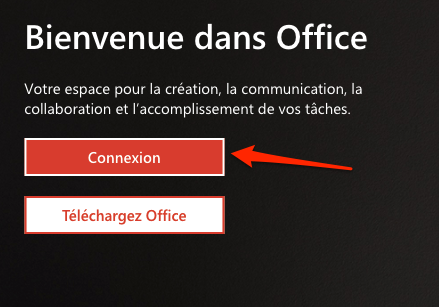
\includegraphics[width=5cm]{./images/teams/ecran_office_com_crop}
\centering
\end{figure}

Vous arrivez sur l'écran de connexion de microsoft office en ligne. Entrez votre adresse mail de l'école (qui se termine donc par \textit{@florimont.ch}).

\begin{figure}[H]
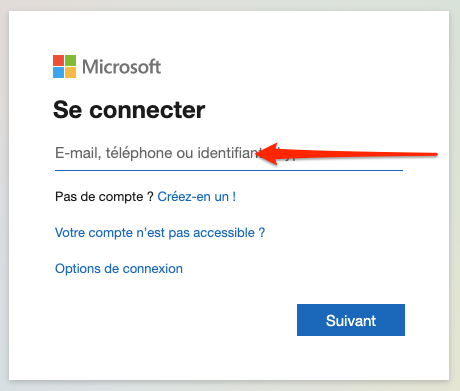
\includegraphics[width=5cm]{./images/teams/ecran_connexion_office_com_crop}
\centering
\end{figure}

Vous êtes alors redirigé vers la page d'identification de l’école. Entrez votre mot de passe. (l'adresse mail est déjà entrée, mais vous pouvez la modifier au cas où vous avez fait une erreur lors de l'étape précédente.)

\begin{figure}[H]
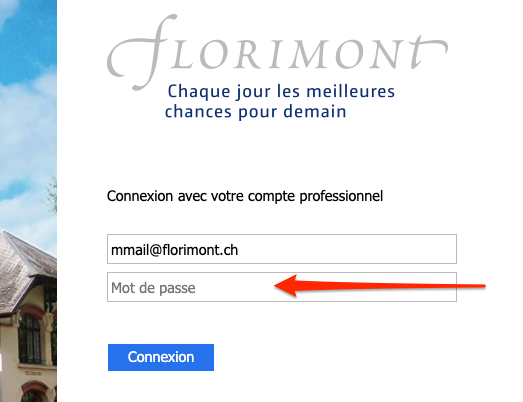
\includegraphics[width=5cm]{./images/teams/ecran_connexion_florimont_crop}
\centering
\end{figure}

Il se peut qu'on vous demande si vous voulez rester connecté. Si vous comptez travailler longtemps sur cette session, il vaut mieux accepter.\\

En revanche, si le navigateur vous propose d'enregistrer votre mot de passe, il est recommandé de refuser (soit en fermant la fenêtre, soit en choisissant \textit{Jamais}). Si vous vous connectez depuis votre ordinateur personnel, il peut être pratique de permettre au navigateur de se souvenir de mots de passe, mais ce n'est jamais une bonne idée sur un ordinateur partagé ou d'emprunt.\\

Le site vous proposera peut-être de télécharger l’application. Cliquez alors sur \textit{Utiliser l’application web à la place}.\\

Alternativement, sur certains navigateurs (comme Safari), vous devrez télécharger l'application de bureau Teams. Cliquez sur \textit{Télécharger l'application} pour continuer.

\begin{figure}[H]
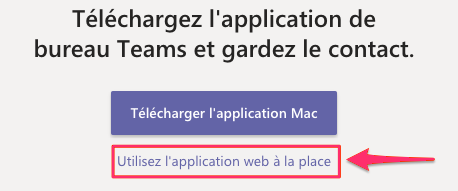
\includegraphics[width=6cm]{./images/teams/ecran_installer_teams_crop}
\centering
\end{figure}

Vous arrivez sur la page de téléchargement de l'application. Cliquez sur \textit{Download Teams}, sous le logo de la pomme, pour télécharger l'application pour Mac.\\

Vous êtes à présent dans votre espace Office. Sur la gauche, choisissez l'icône Teams.

\begin{figure}[H]
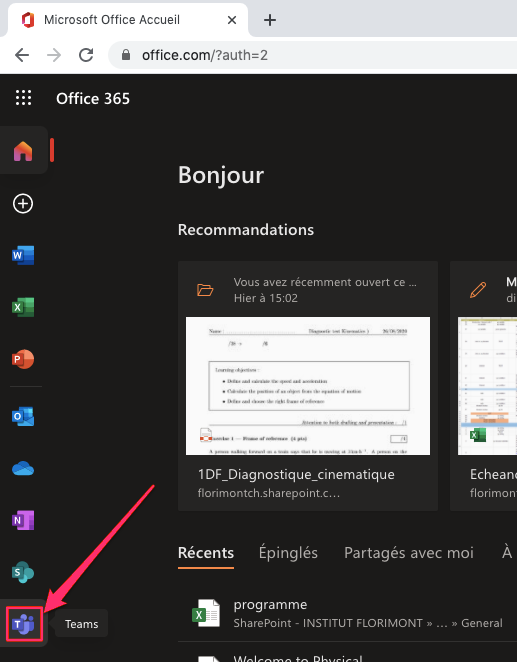
\includegraphics[width=5cm]{./images/teams/ecran_accueil_office_crop}
\centering
\end{figure}

Félicitations, vous arrivez sur la page d'accueil de votre session Teams.




% UTILISATION DE LA PUBLICATION
\section{Utilisation de la Publication}

La messagerie instantanée proposée pour chaque équipe doit permettre aux élèves et aux enseignants de communiquer en dehors de l'école dans un cadre qui reste strictement scolaire. Ainsi les messages personnels n'ont aucune raison d'être sur Teams. Il vous appartient donc de mesurer vos propos lorsque vous utilisez la messagerie instantanée. Ainsi, toute forme d'insulte ou de critique envers un membre de la classe ou une personne extérieure est à proscrire. Le modérateur de chaque équipe est son enseignant responsable.\\

Pour utiliser la messagerie, il suffit de vous rendre sur l'onglet \textit{Publications}

\begin{figure}[H]
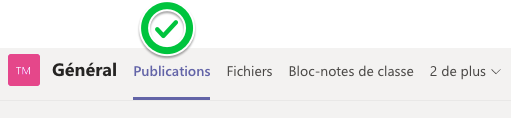
\includegraphics[width=9cm]{./images/teams/publications}
\centering
\end{figure}

puis de rédiger du texte à l'intérieur du champ \textit{Démarrer une conversation}. Utilisez @ pour mentionner un contact, ce qui signifie qu'une notification sera adressée à cette personne. Attention donc de ne pas mentionner un contact inutilement.

\begin{figure}[H]
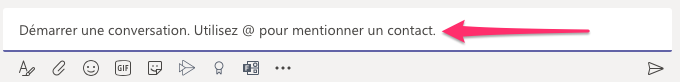
\includegraphics[width=9cm]{./images/teams/publications2}
\centering
\end{figure}

Il ne vous reste plus qu'à cliquer sur l'icône 
\includegraphics[width=0.7cm]{./images/teams/envoi_message} pour envoyer votre message.

\begin{figure}[H]
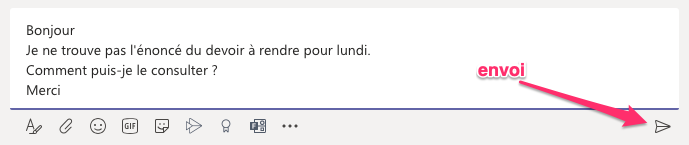
\includegraphics[width=9cm]{./images/teams/publications3}
\centering
\end{figure}





% CONSULTER ET TELECHARGER UN DOCUMENT
\section{Consulter et télécharger un document}

Vous devrez souvent chercher des documents mis en ligne par vos enseignants. Pour faire cela, sélectionnez l'onglet Fichiers, en haut.

\begin{figure}[H]
	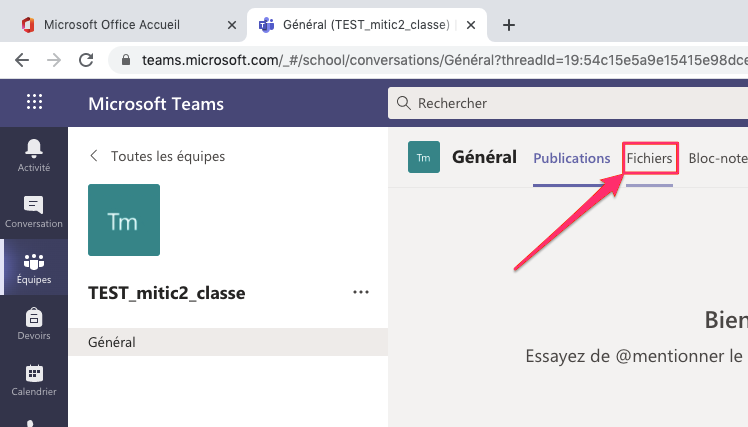
\includegraphics[width=8cm]{./images/teams/accueil_classe_crop}
	\centering
\end{figure}

Les fichiers que vos enseignants mettront à votre disposition seront la plupart du temps rangés dans un dossier. Dans cet exemple, il n'y a qu'un dossier, \textit{Support de cours}. Cliquez dessus pour l'ouvrir.

\begin{figure}[H]
	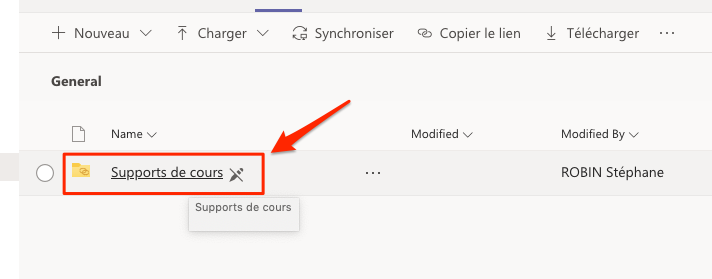
\includegraphics[width=9cm]{./images/teams/ouvrir_dossier_crop}
	\centering
\end{figure}

Vous trouverez dans ce dossier le fichier que votre professeur vous demandera de consulter. Pour le lire, il suffit de cliquer dessus.

\begin{figure}[H]
	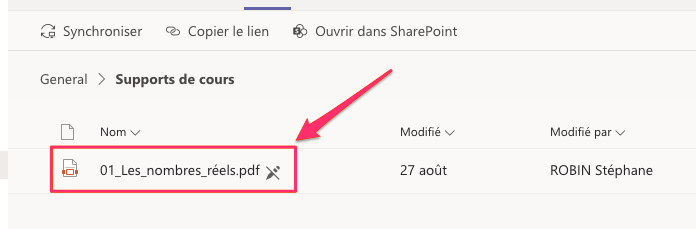
\includegraphics[width=9cm]{./images/teams/ouvrir_fichier_crop}
	\centering
\end{figure}

Vous pouvez à présent consulter le document, mais pas le modifier. Vous pouvez le télécharger pour en garder une copie sur votre ordinateur et éventuellement le modifier par la suite en cliquant sur les trois petits points en haut, puis sur \textit{Télécharger}. Une copie du document apparait alors dans votre dossier Téléchargement.\\

Une fois cela fait, vous pouvez quitter cette page pour revenir à l'affichage du dossier en cliquant sur \textit{Fermer}.
\newpage
\begin{figure}[H]
	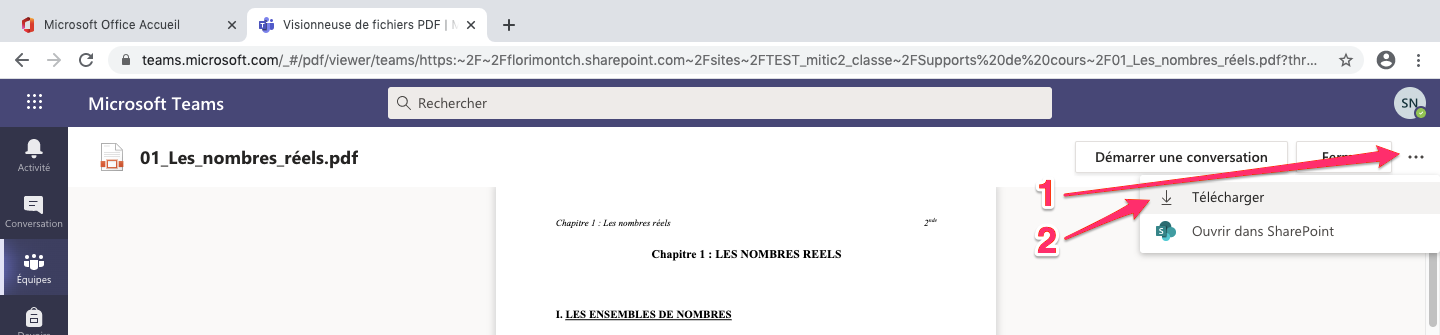
\includegraphics[width=9cm]{./images/teams/telecharger_document_crop}
	\centering
\end{figure}

Il est également possible de télécharger un document depuis la vue du dossier. Il existe plusieurs manières de faire cela. La première consiste à cliquer sur les trois petits points à côté du nom du document, puis sur \textit{Télécharger}.

\begin{figure}[H]
	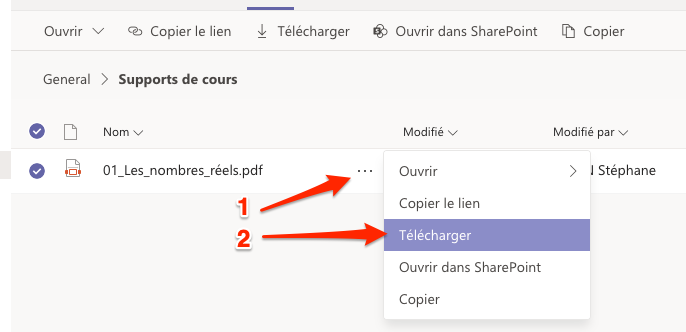
\includegraphics[width=9cm]{./images/teams/telecharger1_crop}
	\centering
\end{figure}

Alternativement, vous pouvez cliquer sur le rond à gauche du nom de fichier pour le sélectionner. Cliquez ensuite sur \textit{Télécharger}, en haut pour télécharger ce fichier. Cette dernière méthode est très pratique si vous désirez télécharger plusieurs fichiers d'un coup, car il suffit alors de les sélectionner puis de cliquer sur \textit{Télécharger} pour les récupérer en même temps.

\begin{figure}[H]
	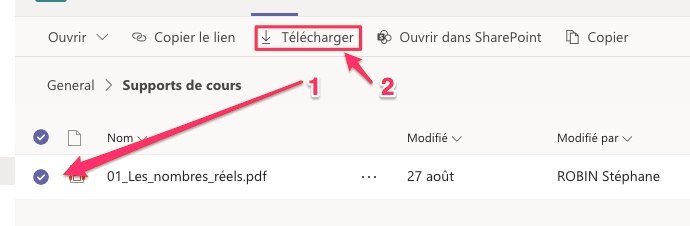
\includegraphics[width=9cm]{./images/teams/telecharger2_crop}
	\centering
\end{figure}



% DEPOSER UN DEVOIR
\section{Les devoirs}

\subsubsection{Consulter le sujet d'un devoir en pièce jointe}\label{consulterDevoir}
Pour consulter les devoirs déposés par votre enseignant, il faut choisir \textit{2 de plus} dans la barre de menus du haut de page, puis sélectionner \textit{Devoirs}.

\begin{figure}[H]
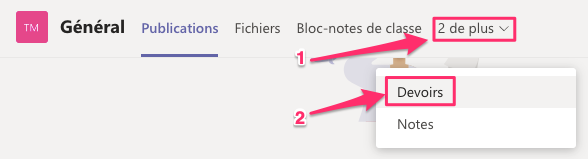
\includegraphics[width=9cm]{./images/teams/devoir1}
\centering
\end{figure}

La page qui s'affiche maintenant fait le bilan de ce qui a déjà été fait et des devoirs proposés par votre enseignant. En cliquant sur \textit{Rédaction} vous pourrez accéder au devoir.

\begin{figure}[H]
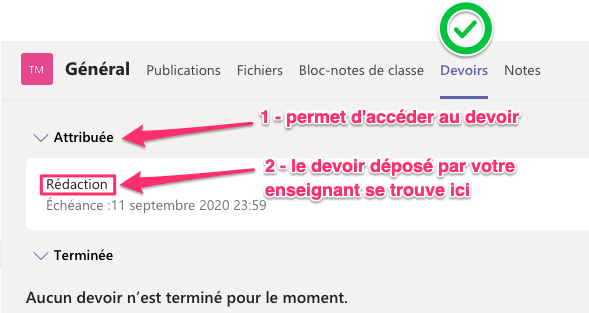
\includegraphics[width=9cm]{./images/teams/devoir2}
\centering
\end{figure}

Vous obtenez alors l'écran suivant

\begin{figure}[H]
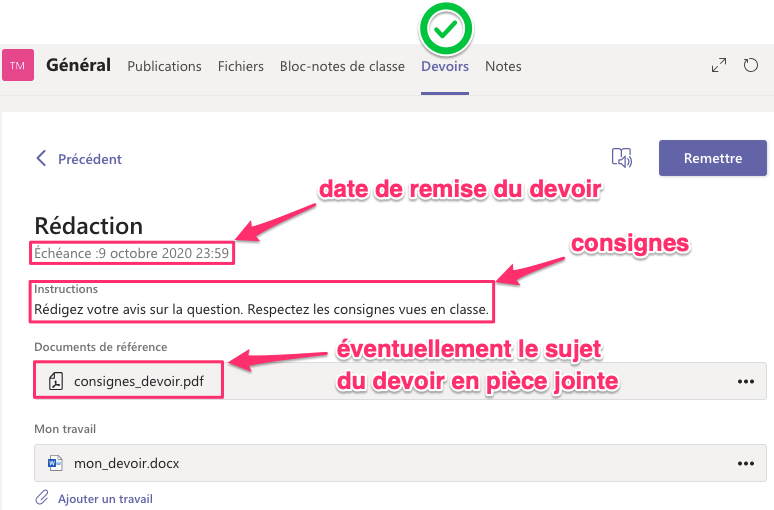
\includegraphics[width=9cm]{./images/teams/devoir3}
\centering
\end{figure}

Il est maintenant possible de consulter le sujet en sélectionnant l'icône 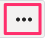
\includegraphics[width=0.7cm]{./images/teams/pointilles} qui vous offre le choix entre une lecture en ligne ou un téléchargement

\begin{figure}[H]
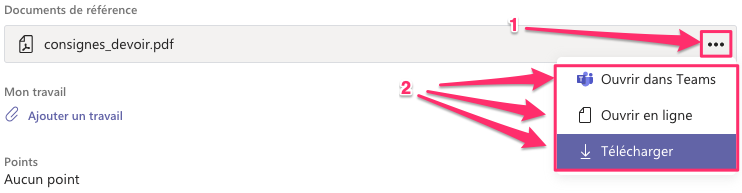
\includegraphics[width=9cm]{./images/teams/choix_pointilles}
\centering
\end{figure}

% REMETTRE SON DEVOIR
\subsection{Remettre son devoir}\label{TeamsRemettreDevoir}

Pour remettre votre devoir, il faut d'abord cliquer sur l'onglet \textit{Ajouter un travail}. 

\begin{figure}[H]
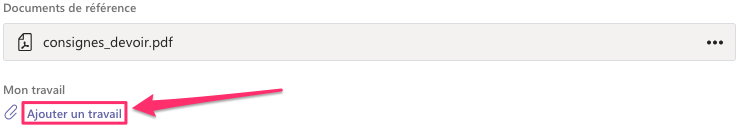
\includegraphics[width=9cm]{./images/teams/ajout}
\centering
\end{figure}

S'ouvre alors une fenêtre qui vous permet de rechercher votre document à partir d'un dossier local relatif à votre ordinateur, à partir du OneDrive ou encore à partir d'une autre équipe.

\begin{figure}[H]
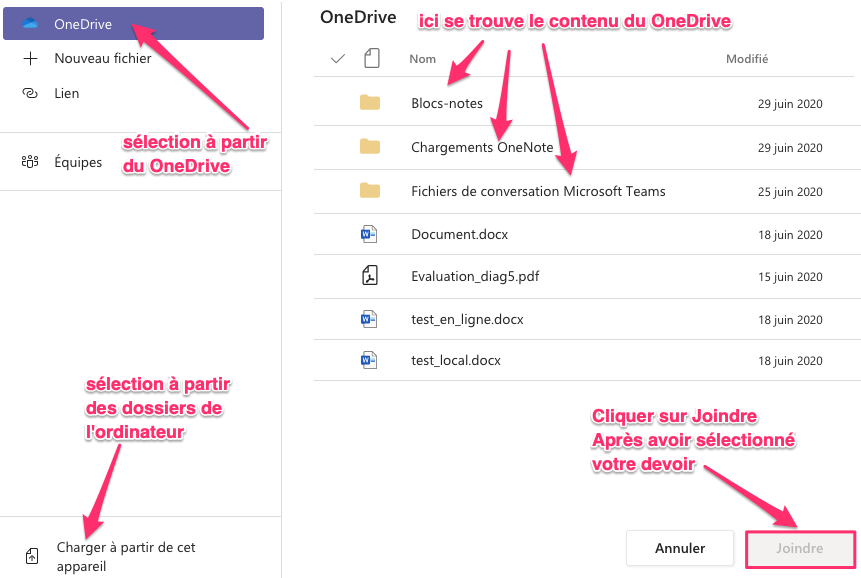
\includegraphics[width=11cm]{./images/teams/selection_devoir}
\centering
\end{figure}

Une fois votre devoir à remettre sélectionné, il suffit de cliquer sur \textit{Joindre}. A ce stade, votre devoir n'est pas encore enregistré. Il faut maintenant choisir \textit{Terminé} pour l'enregistrer.

\begin{figure}[H]
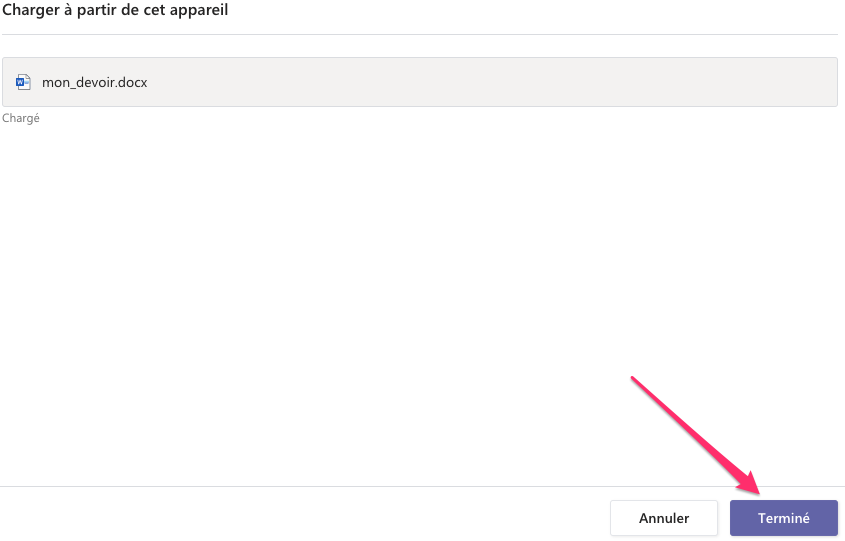
\includegraphics[width=9cm]{./images/teams/ajout2}
\centering
\end{figure}

Vous pouvez également ajouter un autre travail, vous pouvez également télécharger votre devoir afin de vérifier son contenu. Vous pouvez également supprimer votre travail.

\begin{figure}[H]
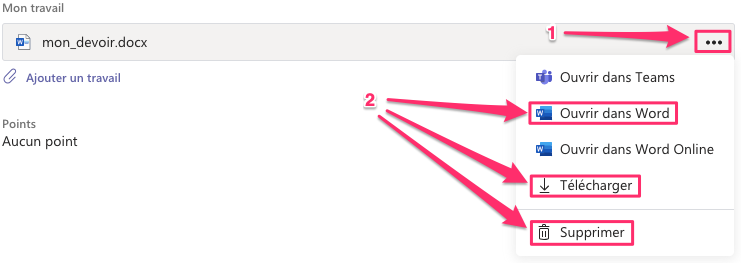
\includegraphics[width=9cm]{./images/teams/ajout3}
\centering
\end{figure}

Attention, votre devoir n'est pas encore remis. il faut maintenant choisir l'onglet \textit{Remettre} pour valider l'envoi de votre devoir. 

\begin{figure}[H]
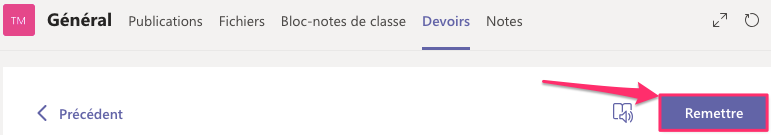
\includegraphics[width=9cm]{./images/teams/ajout4}
\centering
\end{figure}


% ACCEDER A MON CARNET
\section{Accéder à mon bloc-note}

Certains de vos enseignants mettront à votre disposition un bloc-note de classe. C'est un outil très pratique qui permet de prendre des notes et de modifier des fichiers mis à votre disposition, directement depuis Teams.\\

Pour accéder au carnet de classe, cliquez sur \textit{Bloc-notes de classe}, en haut de la page de la classe.

\begin{figure}[H]
	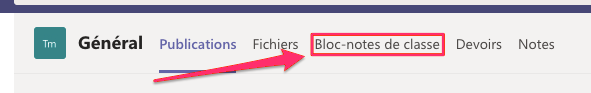
\includegraphics[width=9cm]{./images/teams/acces_bloc_notes_crop}
	\centering
\end{figure}

S'ouvre alors la page d'accueil du bloc-notes. Votre enseignant l'aura probablement adaptée à son cours, elle ne ressemblera donc pas forcément à l'image ci-dessous.

\begin{figure}[H]
	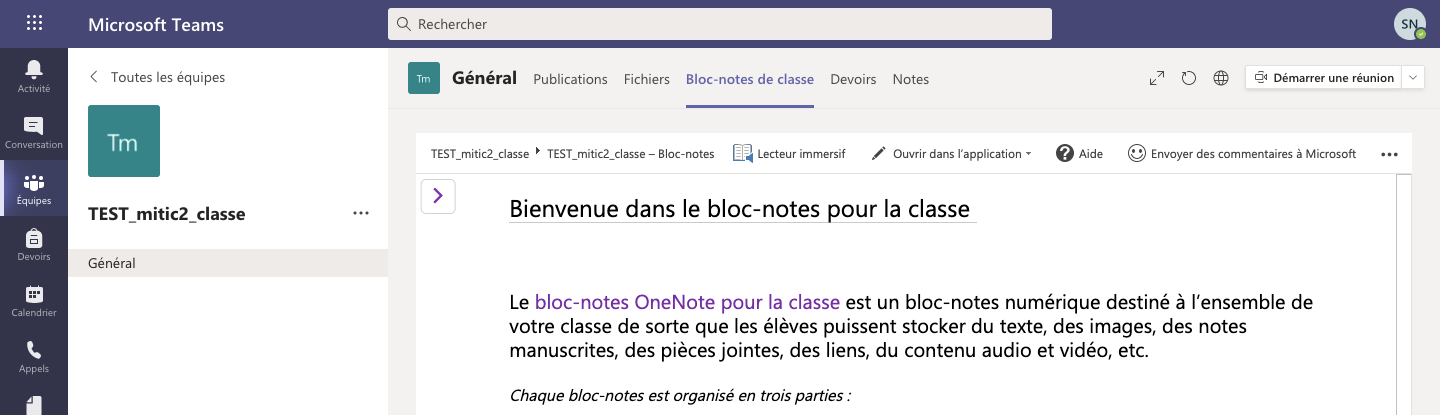
\includegraphics[width=11cm]{./images/teams/ouvrir_menu_bloc_notes_crop}
	\centering
\end{figure}

Cliquez sur la flèche en haut à gauche de l'espace de travail pour ouvrir la liste des bloc-notes. Une section à votre nom apparait, en bas de la liste. Il s'agit d'un espace personnel dans lequel vous pouvez écrire ce que vous voulez, que ce soit pour modifier des fichiers ou prendre des notes. Cliquez sur votre nom pour afficher des sous-sections.

\begin{figure}[H]
	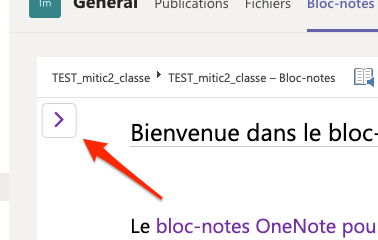
\includegraphics[width=6cm]{./images/teams/ouvrir_liste_dossiers_docs_crop}
	\centering
\end{figure}

Ouvrez la page sans titre, dans la sous-section \textit{Documents}. Ecrivez le titre de votre document. Vous verrez que le titre sera mis à jour dans la liste de documents, à gauche. Si votre liste de sections et documents s'est refermée, il suffit de cliquer sur la flèche, comme tout à l'heure, pour l'afficher à nouveau.\\

Vous pouvez maintenant écrire du texte, ajouter des images, ou modifier ce document comme vous le souhaitez.\\

Si vous souhaitez ajouter une nouvelle page, vous pouvez cliquer sur \textit{+ Page}, en bas. Renommez la nouvelle page en écrivant un titre comme vous venez de le faire.

\begin{figure}[H]
	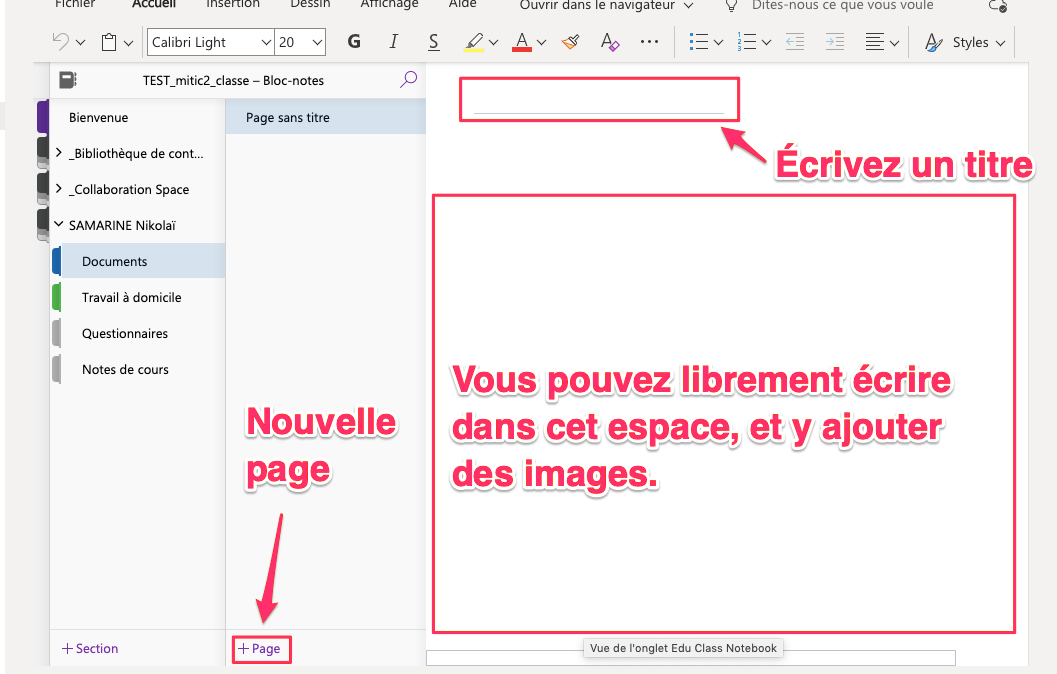
\includegraphics[width=10cm]{./images/teams/sous_section_documents_crop}
	\centering
\end{figure}

En ajoutant et modifiant ainsi des pages, vous allez pouvoir prendre des notes et y accéder via divers appareils, que ce soit depuis la maison ou l'école.

% REJOINDRE UNE VISIO CONFERENCE
\section{Rejoindre une visio-conférence}

Lorsque vous devez assister à un cours à distance, il est nécessaire de rejoindre une visio-conférence déjà commencée. Pour cela, dans l'onglet \textit{Publications}, vous aller trouver une invitation pour participer à une visio-conférence déjà ouverte

\begin{figure}[H]
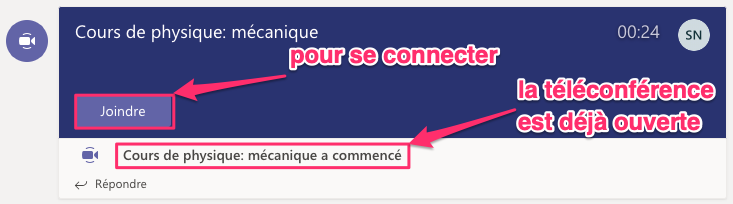
\includegraphics[width=9cm]{./images/teams/video1}
\centering
\end{figure}

Attention, si vous sélectionnez \textit{Demarrer une réunion}, vous allez créer une nouvelle téléconférence et non pas rejoindre la téléconférence déjà programmée pour votre cours.

\begin{figure}[H]
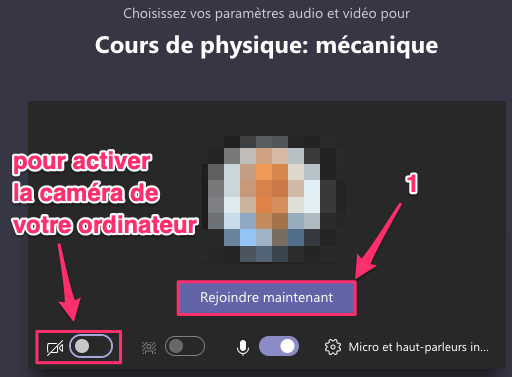
\includegraphics[width=7cm]{./images/teams/video2}
\centering
\end{figure}





% APPARENCE DE LA PAGE D'ACCUEIL
\section{Pour aller plus loin}
\subsection{Apparence de la page d'accueil}

La page d'accueil de Teams se présente sous forme d'une liste d'équipes

\begin{figure}[H]
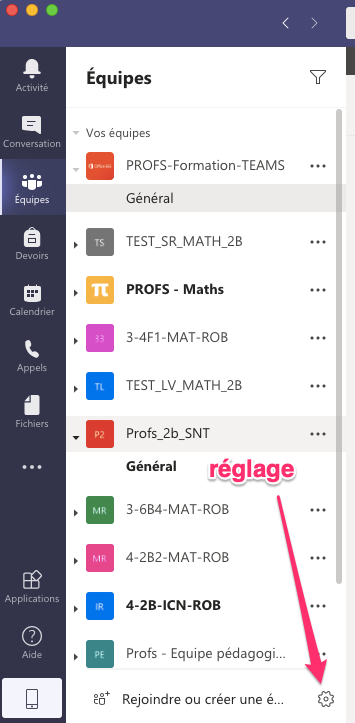
\includegraphics[width=4cm]{./images/teams/accueil_liste}
\centering
\end{figure}

\newpage
ou sous forme d'une grille d'équipes 

\begin{figure}[H]
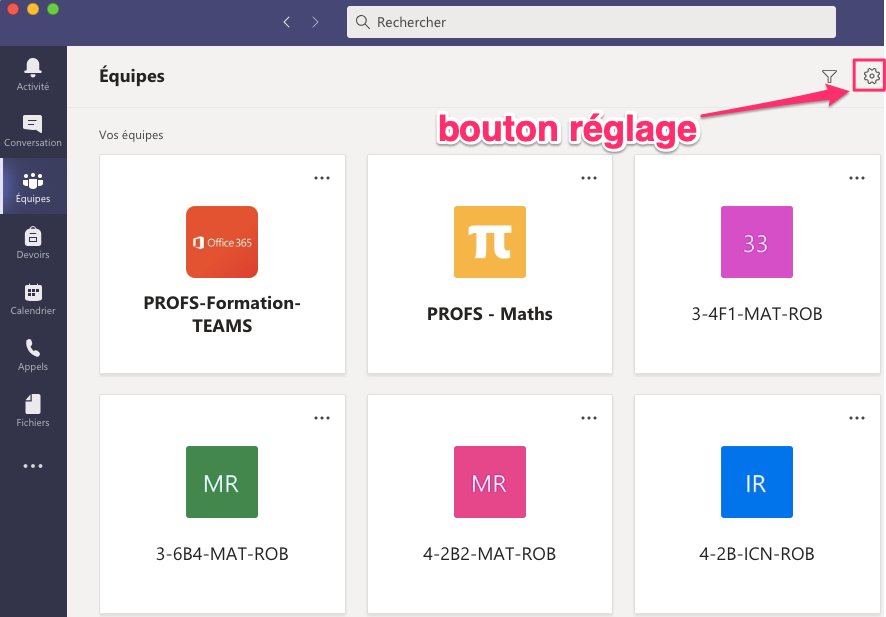
\includegraphics[width=7cm]{./images/teams/accueil_grille}
\centering
\end{figure}

Pour passer d'une forme à l'autre, il faut cliquer sur l'icône 
\includegraphics[width=0.8cm]{./images/teams/bouton_parametres}, choisir \textit{Changer d'affichage} dans le menu déroulant, comme dans l'exemple illustré ci-dessous :

\begin{figure}[H]
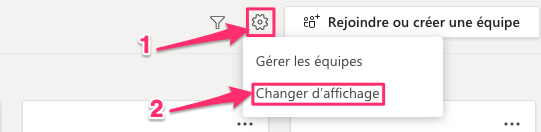
\includegraphics[width=9cm]{./images/teams/changement_liste}
\centering
\end{figure}

Il faut ensuite sélectionner le type d'affichage souhaité entre \textit{Grille} et \textit{Liste}

\begin{figure}[H]
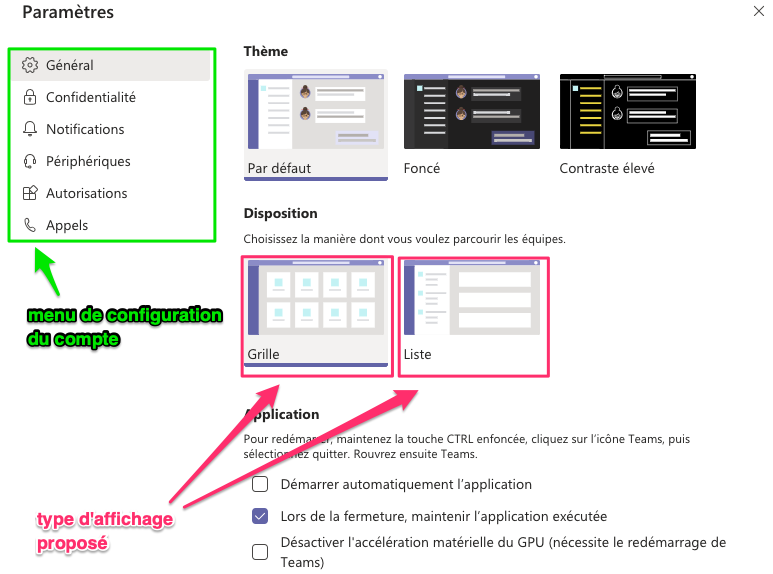
\includegraphics[width=9cm]{./images/teams/choix_parametre}
\centering
\end{figure}

 Pour entrer maintenant dans votre équipe, il suffit de cliquer sur l'icône correspondante

\begin{figure}[H]
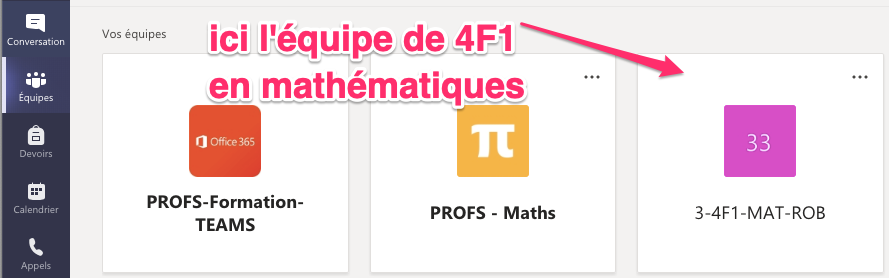
\includegraphics[width=7.5cm]{./images/teams/entree_classe}
\centering
\end{figure}


%\chapter{Tableur}\label{ficheTableur1}  

Un tableur est un logiciel qui permet de faire des calculs à partir de tableaux contenant des nombres (les \emph{données}). Un tableur permet également de représenter ces données sous forme de graphiques qui en facilitent généralement la lecture.\\

\prof{On pourra ici indiquer qu'il existe plusieurs logiciels de tableur, celui que nous allons utiliser étant le plus connu : Excel, contenu dans le pack Office de Microsoft. Un autre tableur très utilisé est Calc, de la suite LibreOffice. Il présente l'avantage d'être libre et gratuit. L'utilisation de nombreuses fonctions est la même pour ces deux logiciels.}

\section*{Synoptique}

{\footnotesize
\begin{itemize}
\item Logiciel : \emph{Microsoft Excel}
\item Prérequis : aucun
\item Matières concernées : mathématiques, physique-chimie, histoire-géographie
\item Objectifs : utiliser un tableur pour traiter des données, les visualiser sous forme de graphique et préparer un compte rendu au format PDF remis sur Teams.
\item Compétences : 
        \begin{itemize}
        \item insérer une formule ;
        \item utiliser la recopie incrémentale ;
        \item tracer un graphique ;
        \item exporter au format PDF.
        \end{itemize}
\item Cette fiche est à réaliser :
        \begin{itemize}
        \item avant les vacances d'octobre en mathématiques ;
        \item avant les vacances de Noël en physique-chimie ;
        \item avant la fin du premier semestre de cours en histoire-géographie. 
        \end{itemize}
\prof{\item vous devez préparer un élément \underline{avant} la séance : un devoir sur Teams où vos élèves déposeront le résultat de leur activité sous la forme d'un fichier PDF.}
\end{itemize}
}


\newpage


\section{Séance 1 : évolution des notes d'un élève}


\subsection{Pour préparer l'activité...}

Voici une présentation vidéo de l'interface graphique de \texttt{Excel}. Pensez à la regarder avant de commencer l'activité de la séance :

\begin{center}
\qrcode[hyperlink, height=0.9in]{https://web.microsoftstream.com/video/aa9246de-61ad-4072-922c-1251a5bd8414}
\end{center}



\subsection{Premiers pas avec Excel...}\index{Ouvrir!Calc}

Il existe trois moyens d'accéder à Excel. La première est de lancer l'application directement. C'est la meilleure méthode car elle donne accès à toutes les fonctionnalités d'Excel. Les autres sont toutefois pratiques si on n'a pas accès à l'application installée. La première alternative est de passer par le site office.com, et l'autre de passer par Teams.

\subsubsection{Lancer l'application Excel}

Lancer le logiciel en utilisant la <<\,loupe\,>> (voir ci-dessous) ou en appuyant simultanément sur cmd et espace :

\uneimageici{./images/generales/loupe}{.7\textwidth}

... puis en indiquant \emph{Excel} :

\uneimageici{./images/tableur/loupe_recherche_Excel1}{.7\textwidth}

Choisir \emph{Microsoft Excel.app} dans la liste proposée :

\uneimageici{./images/tableur/loupe_recherche_Excel2}{.5\textwidth}

On arrive alors dans la fenêtre principale du tableur qui contient une \emph{feuille de calcul} vide :

\uneimageici{./images/tableur/CalcPresentation_Excel_crop}{.9\textwidth}

\subsubsection{Lancer la version en ligne d'Excel}

Ouvrez le navigateur web et allez sur \texttt{office.com}. Cliquez sur le bouton \texttt{Connexion}.

\uneimageici{./images/tableur/ecran_office_com_crop}{.5\textwidth}

Cela ouvre la page de connexion de l'Institut. Entrez votre identifiant et votre mot de passe pour accéder au portail d'office.com. Vous trouverez sur la gauche les boutons menant à toutes les applications d'office. Cliquez sur le logo d'Excel. Cliquez ensuite sur le cadre blanc avec la croix verte pour ouvrir une fenêtre de travail Excel.

\uneimageici{./images/tableur/ecran_office_excel_crop}{.45\textwidth}

\subsubsection{Lancer Excel via Teams}

Si votre enseignant vous a donné un devoir Teams, il se peut qu'il y ait ajouté un fichier que vous pouvez modifier. Pour accéder au devoir, cliquez sur l'onglet \texttt{Devoirs} \circled{1} puis sur le devoir attribué. \circled{2}

\uneimageici{./images/tableur/acces_excel_teams_1_crop}{.6\textwidth}

Une fois dans la page du devoir, vous devriez apercevoir un document excel déjà chargé par votre enseignant. Vous pouvez l'ouvrir en cliquant dessus. Cela ouvre l'interface d'Excel sur Teams.

\uneimageici{./images/tableur/acces_excel_teams_2_crop}{.6\textwidth}

\prof{Faites manipuler les cellules aux élèves, leur faire par exemple remplir la cellule \texttt{AA30} avec un nombre de leur choix, pour qu'ils doivent utiliser les ascenceurs. Montrez aux élèves comment redimensionner une colonne ou une ligne, plusieurs colonnes ou plusieurs lignes (en les sélectionnant auparavant), toutes les colonnes ou toutes les lignes (en les sélectionnant toutes).}

%
%
%  S  É  A  N  C  E     I
%
%


\subsubsection{Pour bien démarrer}

Dès que vous avez ouvert un nouveau document dans \emph{Excel}, sauvegardez-le afin de ne pas le perdre en cas de problème. Pour ce faire, allez dans l'onglet \texttt{Fichier}. \circled{1}

\uneimageici{./images/tableur/office_sauver_1_crop}{.4\textwidth}

Là, cliquez sur \texttt{Enregistrez sous}, à gauche \circled{2}, puis le nouveau \texttt{Enregistrez sous}. \circled{3}

\uneimageici{./images/tableur/office_sauver_2_crop}{.5\textwidth}

Vous pourrez ensuite choisir où enregistrer le fichier (sur onedrive) et quel nom lui donner. Votre fichier devrait être nommé en suivant la logique suivante: Nom-seance1.xlsx, où vous remplacez "NOM" par votre nom (sans espace !).

\subsection{Sujet de l'activité...}

\prof{Assurez-vous que tous les élèves aient franchi les premières étapes ci-dessus. Lire ensuite l'énoncé avec les élèves et montrer le résultat attendu (affichage au TBI du résultat). À partir de ce point, les élèves travaillent chacun à son rythme.}

\boiteEnonce{Au cours d'une année scolaire, un élève a obtenu les notes suivantes sur 20 points : \[11\quad 15\quad 12\quad 18\quad 16\quad 13\quad 8\quad 15\] On souhaite réaliser un graphique qui montre l'évolution de ses notes au cours de l'année et calculer ensuite sa moyenne annuelle. L'objectif est d'obtenir le résultat suivant :
\uneimageici{./images/tableur/CalcSituationFinaleMaths_Excel_crop}{.75\textwidth}
Une fois votre travail terminé, vous devrez exporter (enregistrer sur l'ordinateur) votre fichier au format .xlsx (le fichier doit être nommé à partir de votre nom : \texttt{Nom-seance1.xlsx}) puis vous le rendrez sur Teams à l'endroit indiqué par votre enseignant (si nécessaire, se reporter à la fiche méthode \emph{Remettre son devoir}, page \pageref{TeamsRemettreDevoir}).}

\textbf{Pour obtenir de l'aide, rendez-vous à la page \pageref{aideExcel}}

\subsection{Pour aller plus loin...}

Après avoir terminé, faire des tests :

\begin{itemize}
\item modifier les notes et observer les modifications de la courbe ;
\item exporter le graphique en tant qu'image (sélectionner le graphique, cliquer sur le graphique avec le bouton droit, puis choisir \texttt{Enregistrer en tant qu'image...}) ;\index{Calc!Exporter un graphique comme image}\index{Exporter un graphique comme image (Calc)}
\item mettre en forme la feuille de calcul pour qu'elle ressemble à l'image présentée ci-dessous.
\end{itemize}

\uneimageici{./images/tableur/CalcPourAllerPlusLoin_Excel_crop}{.7\textwidth}

Si vous disposez d'un accès à l'application Excel, vous pouvez exporter votre fichier au format PDF afin que celui-ci puisse être reconnu de manière plus générale.


\newpage

%
%
%  S  É  A  N  C  E     II
%
%




\section{Séance 2 : Suivi en température d'une solidification}\label{ficheTableur2}

\subsection{Pour préparer l'activité...}

Voici une vidéo pour comprendre l'utilité de \texttt{Excel} en comparaison d'une calculatrice. Pensez à la regarder avant de commencer l'activité de la séance :

\begin{center}
\qrcode[hyperlink, height=0.9in]{https://web.microsoftstream.com/video/48370bef-1911-4a74-a09d-6b21e8eb06ea}
\end{center}

\subsection{Pour bien démarrer...}

Dès que vous avez ouvert un nouveau document dans \emph{Excel}, sauvegardez-le au format Nom-seance2.xlsx : dans le menu \texttt{Fichier}, choisir \texttt{Enregistrer sous}.

\uneimageici{./images/generales/clavierCmdS}{.4\textwidth}

\subsection{Sujet de l'activité...}

\prof{réalisez l'expérience avec vos élèves avant la séance, ou apportez le matériel correspondant à l'expérience pour donner du sens à la séance. De même, expliquez aux élèves les résultats obtenus. Il faut bien inciter les élèves à utiliser la recopie incrémentale pour générer les temps de 0 à 10 minutes.}


\boiteEnonce{On place un tube à essai qui contient de l'eau distillée et un thermomètre dans un mélange réfrigérant. 
	\uneimageici{./images/tableur/calcPhyChiSchema}{.4\textwidth}
}

\boiteEnonce{On relève alors la température de l'eau toutes les minutes. Les résultats obtenus sont reportés dans le tableau ci-dessous.
	\begin{center}
		\begin{tabular}{|c|c|c|c|c|c|c|c|c|c|c|c|}
			\hline
			temps $t$ (min) & 0 & 1 & 2 & 3 & 4 & 5 & 6 & 7 & 8 & 9 & 10 \\ \hline
			température $T$ (\degre C) & 15 & 8 & 3 & 0 & 0 & 0 & 0 & 0 & $-1$ & $-3$ & $-5$ \\
			\hline
		\end{tabular}
	\end{center}
	On souhaite réaliser un graphique qui montre l'évolution de la température (en ordonnée) en fonction du temps (en abscisse). Le résultat à obtenir est présenté ci-dessous :
	\uneimageici{./images/tableur/calcPhyChi_Excel}{.7\textwidth}
	Une fois votre travail terminé, vous devrez exporter (enregistrer une copie sur l'ordinateur) votre fichier au format .xlsx (le fichier doit être nommé à partir de votre nom : \texttt{Nom-seance2.xlsx}) et le rendre sur \emph{Teams}.
}

\textbf{Pour obtenir de l'aide, rendez-vous à la page \pageref{aideExcel}}

\subsection{Pour aller plus loin...}

Si vous disposez d'un accès à l'application Excel, vous pouvez exporter votre fichier au format PDF afin que celui-ci puisse être reconnu de manière plus générale.

\newpage



%
%
%  S  É  A  N  C  E     III
%
%




\section{Séance 3 : Évolution de la population mondiale}\label{ficheTableur3}

Voici une vidéo pour comprendre les problèmes simples qu'on peut rencontrer en utilisant \texttt{Excel}. Pensez à la regarder avant de commencer l'activité de la séance :

\begin{center}
\qrcode[hyperlink, height=0.9in]{https://web.microsoftstream.com/video/a6d62817-5809-4e7b-a9c4-0cc79aa37802}
\end{center}

\subsection{Pour bien démarrer...}

Dès que vous avez ouvert un nouveau document dans \emph{Excel}, sauvegardez-le au format Nom-seance3.xlsx : dans le menu \texttt{Fichier}, choisir \texttt{Enregistrer sous}. 

\uneimageici{./images/generales/clavierCmdS}{.4\textwidth}

\subsection{Sujet de l'activité...}

\boiteEnonce{La population mondiale au fil du temps est reportée dans le tableau ci-dessous.
	\newline
	\phantom{rien}
	\newline
	{\footnotesize
		\begin{tabular}{|p{3.5cm}|c|c|c|c|c|c|c|c|c|c|}
			\hline
			Dates (années) & 0 & 400 & 1000 & 1500 & 1700 & 1800 & 1850 & 1900 & 1950 & 1980  \\ \hline
			Population mondiale & \multirow{2}{*}{250} & \multirow{2}{*}{200} & \multirow{2}{*}{300} & \multirow{2}{*}{480} & \multirow{2}{*}{640} & \multirow{2}{*}{900} & \multirow{2}{*}{1300} & \multirow{2}{*}{1700} & \multirow{2}{*}{2700} & \multirow{2}{*}{4400} \\
			(en millions) & & & & & & & & & & \\   
			\hline
		\end{tabular}
		%
		\newline
		\phantom{rien}
		\newline
		%
		\begin{tabular}{|p{3.5cm}|c|c|c|c|c|c|}
			\hline
			Dates (années) & 1990 & 2000 & 2005 & 2010 & 2015 \\ \hline
			Population mondiale & \multirow{2}{*}{5300} & \multirow{2}{*}{6100} & \multirow{2}{*}{6500} & \multirow{2}{*}{6900} & \multirow{2}{*}{7400} \\
			(en millions) & & & & & \\  
			\hline
		\end{tabular}
	} % fin du footnotesize tableau
	%
	\newline
	{\tiny\emph{Source : Wikipédia (Population mondiale) et ONU (World Population Prospects http://esa.un.org/unpd/wpp/)}}
	%
	\newline
	\phantom{rien}
	\newline
	On souhaite représenter l'évolution de la population mondiale depuis le début de notre ère. On veut afficher la population en millions d'individus (en ordonnée) en fonction de l'année (en abscisse).\newline Une fois votre travail terminé, vous devrez exporter (enregistrer sur l'ordinateur) votre fichier au format .xlsx (le fichier doit être nommé à partir de votre nom : \texttt{Nom-seance3.xlsx}) et le rendre sur la Teams.
}

\textbf{Pour obtenir de l'aide, rendez-vous à la page \pageref{aideExcel}}

\prof{cette fois-ci les élèves ne voient pas le graphique à obtenir. Rappelez bien qu'il faut donner des noms aux axes (définir des étiquettes pour les axes), donner un titre au graphique. Interprétez avec les élèves le résultat obtenu. Le graphique que l'on doit obtenir est le suivant :\uneimageici{./images/tableur/calcHistoireGeoGraphique}{.7\textwidth}}

\subsection{Pour aller plus loin...}

Si vous disposez d'un accès à l'application Excel, vous pouvez exporter votre fichier au format PDF afin que celui-ci puisse être reconnu de manière plus générale.

% il faut mettre un calcul de moyenne

% Pour aller plus loin : Europe vs Monde

%
%
%  A  I  D  E
%
%

\newpage

\section{Aide pour réaliser les activités}\label{aideExcel}

\subsubsection{Entrer les données}

\begin{itemize}
\item Cliquer dans la cellule \texttt{A1}.
\item Taper au clavier le texte qui doit être contenu dans la cellule : \texttt{numéro du test}.
\item Cliquer dans la cellule \texttt{B1} et écrire le premier numéro du test : 1.
\item Cliquer dans la cellule \texttt{C1} et écrire le deuxième numéro du test : 2.
\item Utiliser la \emph{recopie incrémentale}\index{Recopie incrémentale (Calc)}\index{Calc!Recopie incrémentale} pour remplir les cellules suivantes : pour cela, sélectionner les deux cellules (B1 et C1). Approcher le curseur de la souris du coin inférieur droit de la cellule \texttt{C1}. Lorsque le curseur se change en croix
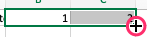
\includegraphics[scale=.4]{./images/tableur/recopieIncrementale_Excel_crop}, cliquer et tirer (en maintenant cliqué) vers la droite pour remplir les cellules suivantes jusqu'à la valeur 8 (voir image ci-dessous).
\end{itemize}

\uneimageici{./images/tableur/recopieIncrementale_Excel2_crop}{\textwidth}

\begin{itemize}
\item Cliquer dans la cellule \texttt{A2} et écrire \texttt{note sur 20}.
\item Remplir les cellules de la ligne 2 avec les notes correspondant aux différents tests.
\end{itemize}





\subsubsection{Sauvegarder le fichier}
\label{ssec_sauvegarder_fichier}
Il est important de sauvegarder régulièrement le fichier sur lequel on travaille. Sur la version en ligne d'\emph{Excel}, cela se fait automatiquement à partir du moment où le fichier a été enregistré une première fois.


Pour enregistrer votre travail sur la version logicielle d'\emph{Excel} :
\begin{itemize}
\item Ouvrir le menu \texttt{Fichier}.
\item Choisir \texttt{Enregistrer sous...}
\item Entrer le nom du fichier sous la forme \texttt{Nom-date}. \circled{1} comme dans l'exemple ci-dessous
\item Cliquer sur \texttt{Sur mon Mac} pour choisir où enregistrer le fichier. Cela transforme la fenêtre. \circled{2}
\item Choisir comme emplacement le \emph{Bureau} de l'ordinateur. \circled{3}
\item Vérifier que le fichier est bien enregistré au format \emph{Classeur Excel (.xlsx)}. \circled{4}
\end{itemize}

\uneimageici{./images/tableur/CalcEnregistrerFichier_Excel1_crop}{.7\textwidth}

\uneimageici{./images/tableur/CalcEnregistrerFichier_Excel2_crop}{.9\textwidth}

Une fois cela fait, appuyer régulièrement sur la combinaison de touche \texttt{cmd} + \texttt{S} : c'est le \emph{raccourci clavier} permettant d'enregistrer votre travail.

\uneimageici{./images/generales/clavierCmdS}{.5\textwidth}



\cadre{\textbf{Différence entre \texttt{Enregistrer} et \texttt{Enregistrer sous...}}\newline Dans la plupart des logiciels, on peut : \begin{itemize}\item \textbf{Enregistrer} le fichier sur lequel on travaille. Cette opération est possible si le fichier existe déjà et possède un nom. La version courante du fichier sera alors sauvegardée et remplacera l'ancienne version du fichier.
\item \textbf{Enregistrer sous...} le fichier sur lequel on travaille. Cette opération commence par demander un nouveau nom pour l'enregistrement du fichier. On peut donc ouvrir un fichier que l'on ne souhaite pas modifier, choisir \emph{enregistrer sous}, donner un nouveau nom et ainsi travailler sur une copie du fichier de départ.
\item utiliser \texttt{cmd + s} (\emph{s} pour \emph{Save}) pour \textbf{enregistrer} le fichier courant. Bien que les documents soient enregistrés automatiquement par la majorité des logiciels, il faut régulièrement sauver son travail pour éviter les surprises.\end{itemize}}









\subsubsection{Créer un graphique}\index{Calc!Créer un graphique}\index{Créer un graphique (Calc)}

\begin{itemize}
\item Sélectionner les données à représenter : cliquer sur la cellule \texttt{B1} sans relâcher le bouton et tirer (en maintenant cliqué) jusqu'à la cellule \texttt{I2}. Les cellules sélectionnées apparaissent en gris.
\uneimageici{./images/tableur/CalcCellulesSelectionnees_Excel_crop}{.9\textwidth}

\item Cliquer alors sur l'onglet \texttt{Insertion}\circled{1} puis sur la flèche à côté des icônes de graphiques pour voir la liste de tous les types de graphiques disponibles \circled{2}. Cliquez enfin sur l'image représentant le type de graphique souhaité. Dans notre cas, ce sera un graphique en nuage de points. \circled{3}
\uneimageici{./images/tableur/CalcBoiteDiagramme1_oExcel_crop}{.9\textwidth}
\end{itemize}

Vous avez maintenant un graphique qui s'est ajouté dans la feuille de calcul. Attention, la fenêtre du graphique est sélectionnée, ce qui est visible grâce aux huit poignées de sélection qui entourent la fenêtre :

\uneimageici{./images/tableur/CalcFenetreGraphiqueSelectionnee_oExcel_crop}{.6\textwidth}

Pour déplacer la fenêtre graphique, déplacer la souris sur le bord pour qu'apparaisse sur le curseur une croix. Le déplacement s'effectue en maintenant cliqué et en déplaçant la souris. Pour revenir à la feuille de calcul, cliquer sur n'importe quelle cellule (les poignées de sélection disparaissent alors).


Pour ajouter des titres aux axes, il faut d'abord sélectionner le graphique (à nouveau, vérifiez que les poignées de sélection sont bien présentes autour de celui-ci) et cliquer sur \texttt{Titres des axes} dans l'onglet \texttt{Graphique}. \circled{1} Choisir ensuite l'axe pour lequel on veut ajouter un titre (exemple ici : l'axe horizontal : \circled{2}) et enfin l'option pour faire apparaitre un titre. \circled{3}

\uneimageici{./images/tableur/Calc_office_ajouter_titres_axes_crop}{.6\textwidth}

Une fenêtre s'ouvre alors, vous demandant d'écrire le titre qui va ensuite apparaître. Cliquez sur \texttt{OK} lorsque le titre vous convient.

Pour modifier le titre d'un axe ou le supprimer, les options pour ce faire apparaissent au même endroit où on a cliqué pour ajouter un axe, mais il faut choisir les options \texttt{Modifier le titre de l'axe horizontal...} (ou vertical) ou \texttt{Aucun} à la place de celle qui a ajouté un titre.


\subsubsection{Calculer la moyenne}\index{Moyenne (calcul de la)}\index{Calc!Moyenne (calcul de la)}

\begin{itemize}
\item cliquer dans la cellule \texttt{A4} et entrer le texte : \texttt{Moyenne}. \circled{1}
\item cliquer dans la cellule \texttt{B4} dans laquelle nous allons entrer une formule : \circled{2}
        \begin{itemize}
        \item taper un signe \texttt{=} qui signifie que la cellule va contenir une formule ;
        \item taper le nom de la formule suivie d'une parenthèse ouvrante : \texttt{=MOYENNE(} ;
        \item à l'aide de la souris, sélectionner dans la feuille de calcul les cellules contenant les notes dont on veut calculer la moyenne (voir image ci-dessous \circled{3}) ;
        \uneimageici{./images/tableur/CalcCalculMoyenne_Excel_crop}{.8\textwidth}
        \item appuyer sur la touche \texttt{Entrée} : la moyenne calculée apparaît.
        \end{itemize}
\end{itemize}



\subsubsection{Exporter au format PDF}\index{Calc!Exporter au format PDF}\index{PDF (exporter au format) (Calc)}

Une fois le travail achevé et sauvegardé, il faut exporter le fichier au format PDF. Pour cela, il faut passer par le menu \texttt{Fichier} et choisir \texttt{Imprimer} \circled{1} puis \texttt{Imprimer} \circled{2} comme si vous vouliez imprimer votre fichier.

\uneimageici{./images/tableur/Exporter_PDF_office_1_crop}{.4\textwidth}

S'ouvre alors un aperçu de votre document avec, à droite, quelques paramètres qui permettent notamment de changer l'échelle ou l'orientation de la page. Nous n'allons pas toucher à ces options et simplement nous contenter de cliquer sur le bouton \texttt{Impression}, en bas.

\uneimageici{./images/tableur/Exporter_PDF_office_2_crop}{.4\textwidth}

Il se peut que l'on vous demande une confirmation : dites alors que vous êtes sûrs que la page doit bien être imprimée. Vous allez voir c'est à cette étape que nous allons indiquer qu'il faut en réalité exporter le document au format PDF.

Dans la fenêtre qui apparaît, qui permet habituellement, de communiquer les réglages à l'imprimante, cliquer sur le bouton \texttt{PDF}, en bas à gauche. \circled{1} Parmi les options qui apparaissent, sélectionner \texttt{Enregistrer au format PDF}. \circled{2}

\uneimageici{./images/tableur/Exporter_PDF_office_3_crop}{.4\textwidth}

Vous pouvez ensuite choisir où vous désirez exporter votre nouveau fichier PDF. Faites attention à vous souvenir de l'endroit où vous l'enregistrez, car vous allez en avoir besoin plus tard.

\cadre{Le \textbf{format PDF} est un format parfaitement adapté aux échanges de documents : il est non modifiable et lisible sur tous les périphériques (ordinateurs, tablettes, smartphones). Il peut contenir du texte, des images, des liens vers l'internet et même des vidéos ou du son. \newline À chaque fois qu'il faut rendre ou envoyer un document qui n'est pas destiné à être modifié, il faut privilégier le format de fichier PDF.}

Sur l'application \emph{Excel}, il est également possible de n'exporter qu'un graphique au format PDF. Dans ce cas, il faut cliquer une fois sur le graphique puis cliquer droit dessus et choisir \texttt{Enregistrer en tant qu'image...}. S'ouvre alors la fenêtre ci-dessous.

\uneimageici{./images/tableur/Exporter_graphique_PDF_crop}{.7\textwidth}

En bas, sélectionnez le type de fichier souhaité (PDF). \circled{1} Cela met à jour l'extension du fichier dans la barre en haut de la fenêtre. \circled{2} Pour le reste, cela fonctionne de la même manière que précédemment.



\subsubsection{Remettre le travail achevé sur Teams}

Une fois le travail terminé et exporté au format PDF, il faut le remettre au professeur. Pour cela, se connecter à Teams et accéder à l'équipe du cours. Cliquer sur \texttt{Devoirs} et cliquez sur le devoir correspondant à l'activité que vous êtes en train de terminer. Cliquez sur \texttt{Ajouter un travail}, en bas, puis \texttt{Charger à partir de cet appareil}, en bas à gauche. Sélectionnez le fichier au format PDF que vous venez d'exporter et \texttt{Ouvrir}. Une fois le travail chargé, cliquez sur \texttt{Terminé}, en bas à droite. Enfin, cliquez sur \texttt{Remettre}, en haut à droite.\\



Si nécessaire, se reporter à la fiche méthode \emph{Remettre un devoir sur Teams}, page \pageref{TeamsRemettreDevoir}.



\poubelle{


}
\chapter{Traitement de texte}\label{ficheTexte1}  

Un traitement de texte est un logiciel qui permet d'effectuer la mise en forme d'un texte : choix d'une police de caractères, de sa taille, de sa couleur, mise en forme de la page, des marges, des pieds de page, des entêtes, mise en forme des paragraphes, création de listes à puces, de listes numérotées, ou encore toute fonctionnalité permettant de personnaliser le contenu d'un document.\\

\prof{on pourra ici indiquer qu'il existe plusieurs logiciels de traitement de texte, le plus connu étant Word contenu dans le pack Office de Microsoft. Le traitement de texte utilisé ici est Writer, de la suite LibreOffice. Il présente l'avantage d'être libre et gratuit. L'utilisation de nombreuses fonctions est la même pour ces deux logiciels.}

{\footnotesize
\begin{itemize}
\item Logiciel\footnote{Le logiciel Microsoft Word est téléchargeable à l'adresse suivante : \url{https://www.microsoft.com/fr-ch/microsoft-365/microsoft-office?rtc=1}. Il s'agit d'un logiciel propriétaire qui nécessite une licence pour être exploité.} : \emph{Microsoft Word} 
\item Prérequis : aucun
\item Matières concernées : français, anglais, sciences de la Vie et de la Terre
\item Objectifs : utiliser un traitement de texte pour mettre en forme un texte simple et l'exporter au format PDF (les documents seront rendus sur la plateforme \emph{Teams}).
\item Compétences : 
        \begin{itemize}
        \item distinguer et mettre en forme caractères, paragraphes et pages ;
        \item insérer une image ; 
        \item exporter au format PDF.
        \end{itemize}
\item Cette fiche est à réaliser :
        \begin{itemize}
        \item avant les vacances d'octobre en français ;
        \item avant les vacances de Noël en anglais ;
        \item avant les vacances de printemps en sciences de la Vie et de la Terre. 
        \end{itemize}
\prof{\item vous pourriez préparer trois éléments \underline{avant} la séance : \begin{itemize}\item récupérer sur Teams le fichier qui contient un texte simple non mis en forme sur lequel les élèves travailleront ;\item mettre à disposition des élèves sur la page Teams de votre cours le fichier sur lequel ils travailleront ; \item créer un dossier de remise de devoir sur la page Teams de votre classe car les élèves rendent cette activité sous la forme d'un fichier PDF déposé sur Teams.\end{itemize} }
\end{itemize}
}






\newpage





%
%
%  S  É  A  N  C  E     I
%
%




\section{Séance 1 : mise en forme de \emph{La Belle et la Bête}}\index{Writer!Mise en forme simple d'un texte}\index{Mise en forme d'un texte (Writer)}

\subsection{Premiers pas avec Word}\index{Ouvrir!Writer}

Lancer le logiciel en utilisant la <<\,loupe\,>> :

\uneimageici{./images/generales/loupe}{.7\textwidth}

... puis en indiquant \emph{Word} :

\uneimageici{./images/texte/loupeRecherche}{.7\textwidth}

Choisir \emph{Microsoft Word.app} dans la liste proposée :

\uneimageici{./images/texte/WordOuverture}{.6\textwidth}

La fenêtre suivante propose de choisir entre :
\begin{itemize}
\item un onglet \emph{Nouveau}, permettant de commencer avec un document vide,
\item un onglet \emph{Récent}, qui propose les derniers documents enregistrés,
\item un onglet \emph{Partagé}, lié à des documents présents sur le drive,
\item un onglet \emph{Ouvrir}, permettant d'accéder à un document enregistré.
\end{itemize}

\uneimageici{./images/texte/WordPresentation}{.7\textwidth}

On arrive alors dans la fenêtre principale du traitement de texte qui contient une page blanche. Les principales icônes sont décrites ci-dessous :

\uneimageici{./images/texte/WriterPresentation}{\textwidth}

\prof{faites manipuler le logiciel aux élèves, parcourez avec eux les différentes icônes.}





\subsection{Pour bien démarrer...}

Sur la page \emph{Fichiers} de Teams, récupérer le fichier \texttt{LaBelleEtLaBete.docx}. Si nécessaire, se reporter à la fiche méthode \emph{Consulter et télécharger un document} sur Teams.\\

Une fois le fichier enregistré sur le \emph{Bureau} de l'ordinateur, revenir dans \emph{Microsoft Word}, cliquer sur l'onglet \emph{Ouvrir}. Vous pouvez également choisir d'enregistrer votre fichier sur votre \emph{OneDrive} personnel, si vous souhaitez conserver votre travail en vue de l'utiliser à la maison par exemple.

\uneimageici{./images/texte/ouvrirDoc1.png}{.5\textwidth}

A l'emplacement de \texttt{Mon ordinateur} ou \texttt{Sur mon Mac} \circled{1}, choisir \texttt{Bureau} \circled{2}, puis cliquer sur le nom du fichier \circled{3} avant d'appuyer sur le bouton \texttt{Ouvrir} \circled{4}.      

\uneimageici{./images/texte/ouvrirDoc2.png}{.9\textwidth}





Il est important de sauvegarder régulièrement le fichier sur lequel on travaille.

Pour enregistrer votre travail :
\begin{itemize}
\item Ouvrir le menu \texttt{Fichier}.
\item Choisir \texttt{Enregistrer sous...} \circled{1}
\item Choisir comme emplacement le \emph{Bureau} \circled{2} de l'ordinateur.
\item Entrer le nom du fichier sous la forme \texttt{Nom-date.docx}
\item Sélectionner \texttt{Enregistrer} \circled{3}
\end{itemize}

\uneimageici{./images/texte/ouvrirDoc3.png}{.8\textwidth}

Appuyer régulièrement sur la combinaison de touche \texttt{cmd} + \texttt{S} : c'est le \emph{raccourci clavier} permettant d'enregistrer votre travail.\index{Raccourci Clavier! Cmd + S, enregistrer}

\uneimageici{./images/generales/clavierCmdS}{.5\textwidth}


\subsection{L'activité demandée}

\vspace{10pt}

\prof{Assurez-vous que tous les élèves ont franchi les premières étapes ci-dessus. Lire ensuite l'énoncé avec les élèves et montrer le résultat attendu (affichage au TBI du résultat). À partir de ce point, les élèves travaillent chacun à leur rythme.}

\boiteEnonce{Le but de cette activité est de mettre en forme un extrait de \emph{La Belle et la Bête}, de Jeanne-Marie Leprince de Beaumont, dont vous venez de récupérer une version <<\,brute\,>> sur \emph{Teams}. Vous chercherez à reproduire le résultat ci-dessous par vous-mêmes, en testant les différentes icônes de l'interface de Word. C'est encore la meilleure façon de se familiariser avec cette application.\\ \\
Vous veillerez à utiliser une marge de 4 cm à droite et à gauche, ainsi que de 3 cm en haut et en bas de la page. La police de caractère choisie est ``Times New Roman'', avec une taille de 12 points pour les paragraphes et de 16 points pour le titre.\\ \\
Une fois la mise en forme terminée, vous exporterez votre fichier au format PDF (le fichier doit être nommé à partir de votre nom : \texttt{Nom-date.pdf}), puis vous le rendrez sur \emph{Teams} à l'endroit indiqué par votre enseignant. (si nécessaire, se reporter à la fiche méthode \emph{Remettre son devoir}, page \pageref{TeamsRemettreDevoir}} 

\vfill
\phantom{rien}

\begin{center}\fbox{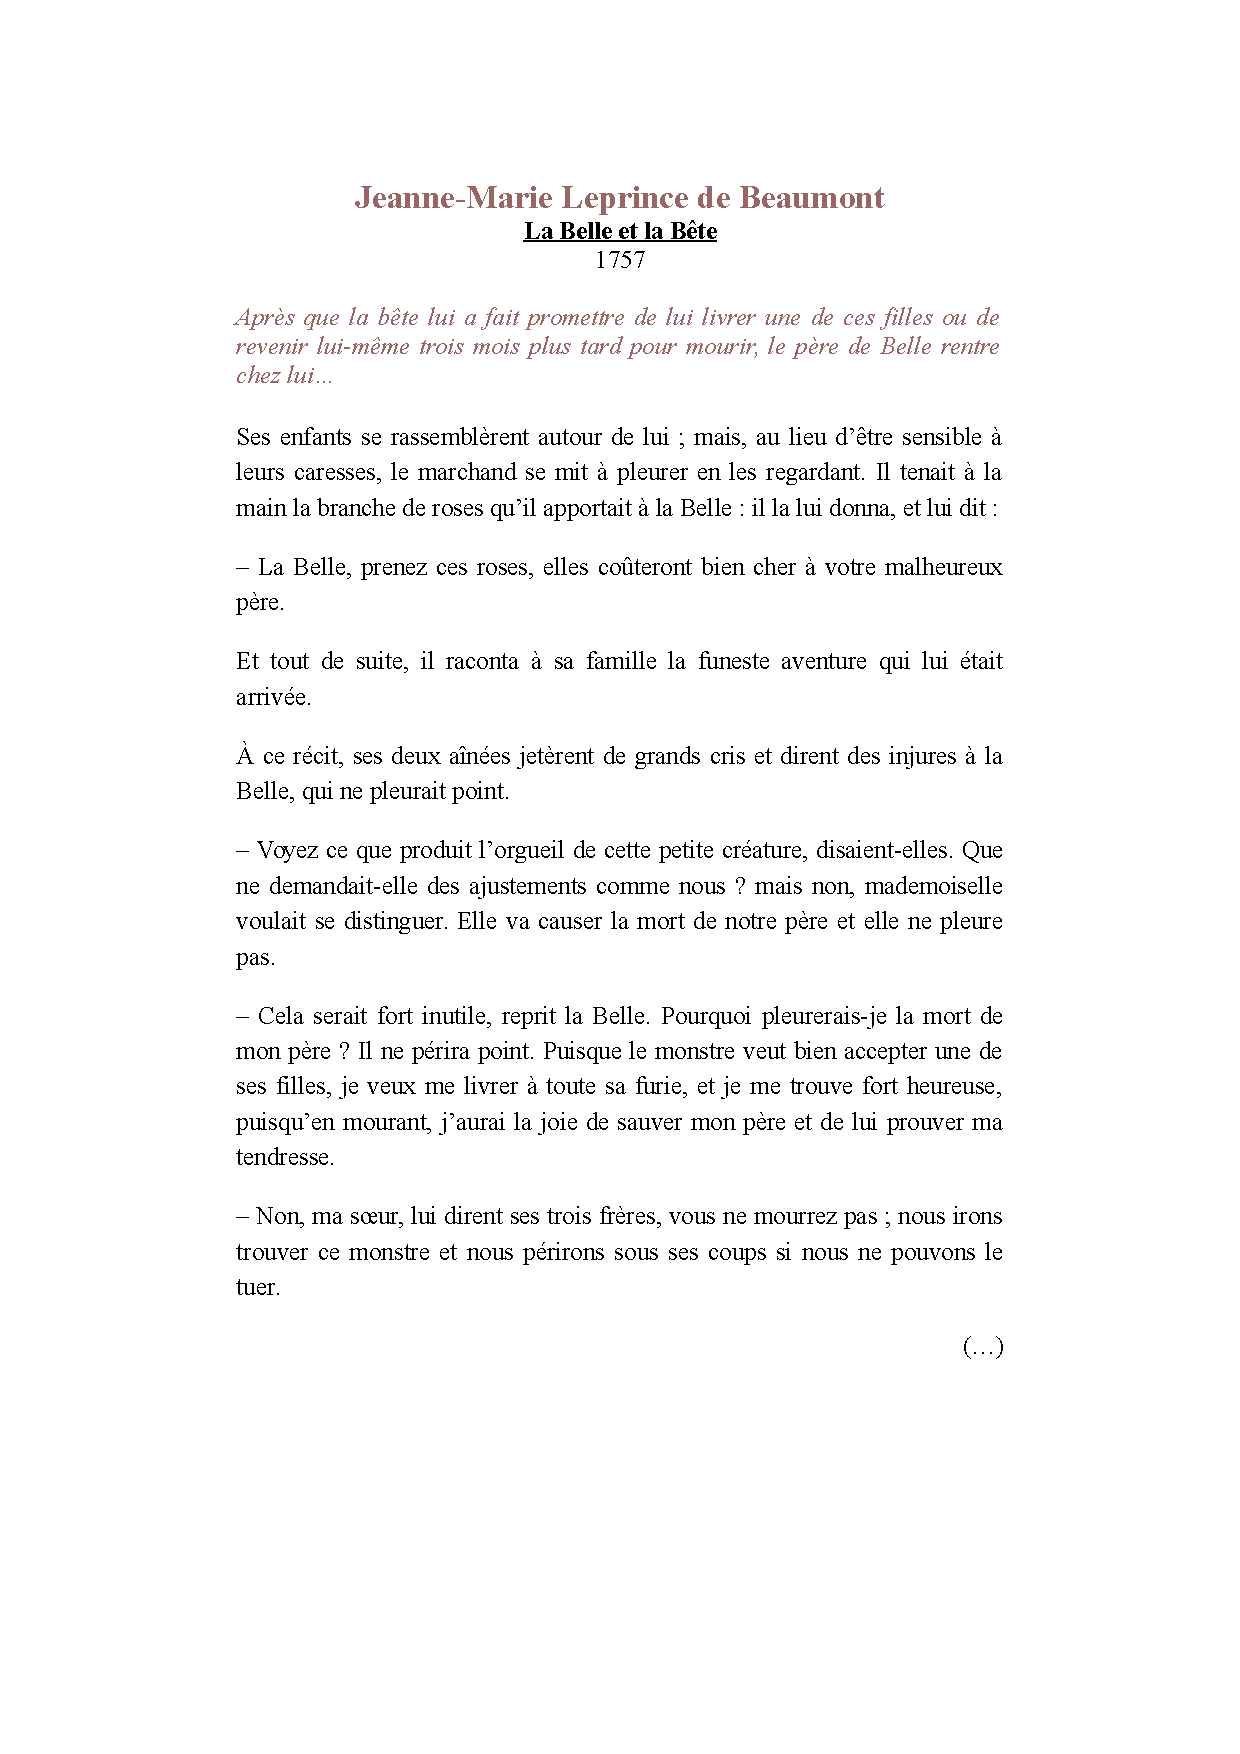
\includegraphics[width=.8\textwidth]{./sources/texte01/LaBelleEtLaBeteFormatee}}\label{modelePage}\end{center}



\textbf{Pour obtenir de l'aide, rendez-vous à la page \pageref{correction_texte01}}


\subsection{Pour aller plus loin...}  

Quand les textes deviennent très longs, il est difficile d'y retrouver un mot en particulier. Les traitements de texte disposent donc d'un outil permettant de rechercher un mot.\index{Writer!Rechercher}\index{Rechercher (Writer)} 

Lorsqu'on souhaite retrouver un mot dans une page de texte, on peut utiliser le raccourci clavier \texttt{cmd + F} :\index{Raccourci Clavier! Cmd + F, rechercher (Writer)}   

\uneimageici{./images/generales/clavierCmdF}{.35\textwidth}

Une barre de recherche s'ouvre alors en haut de la fenêtre :

\uneimageici{./images/texte/WordBarreRecherche.png}{.9\textwidth}

Essayez de rechercher le mot \emph{Belle} : il suffit d'entrer le mot dans la zone de saisie, puis d'appuyer sur la touche \texttt{Entrée}. Pour fermer la barre de recherche, utilisez de nouveau le raccourci clavier \texttt{cmd + F}.   










\poubelle{


%
%
%  S  É  A  N  C  E     II
%
%


\section{Séance 2 : mise en forme d'un texte de J. Swift}\label{ficheTexte2}

\subsection{L'activité demandée}

\prof{l'anglais est enseigné en groupes de niveau et il était difficile de trouver un texte qui soit valable pour tous les groupes. N'hésitez pas à vous approprier cette séance en proposant votre propre texte à votre groupe. Si vous souhaitez faire cette activité avec un texte différent, il suffit de fournir aux élèves (i) le texte brut non mis en forme, (ii) le modèle à atteindre. Ainsi vous pourrez mieux intégrer cette séance à votre progression.}  



\boiteEnonce{Le but de cet exercice est de mettre en forme un extrait d'une œuvre de Jonathan Swift, \emph{Gulliver's travels}, dont une version <<\,brute\,>> est disponible sur la page \emph{Teams} de votre cours. Le modèle à obtenir est montré ci-dessous. Essayez par vous-mêmes de trouver comment faire en testant les possibilités du logiciel.}


\begin{center}\fbox{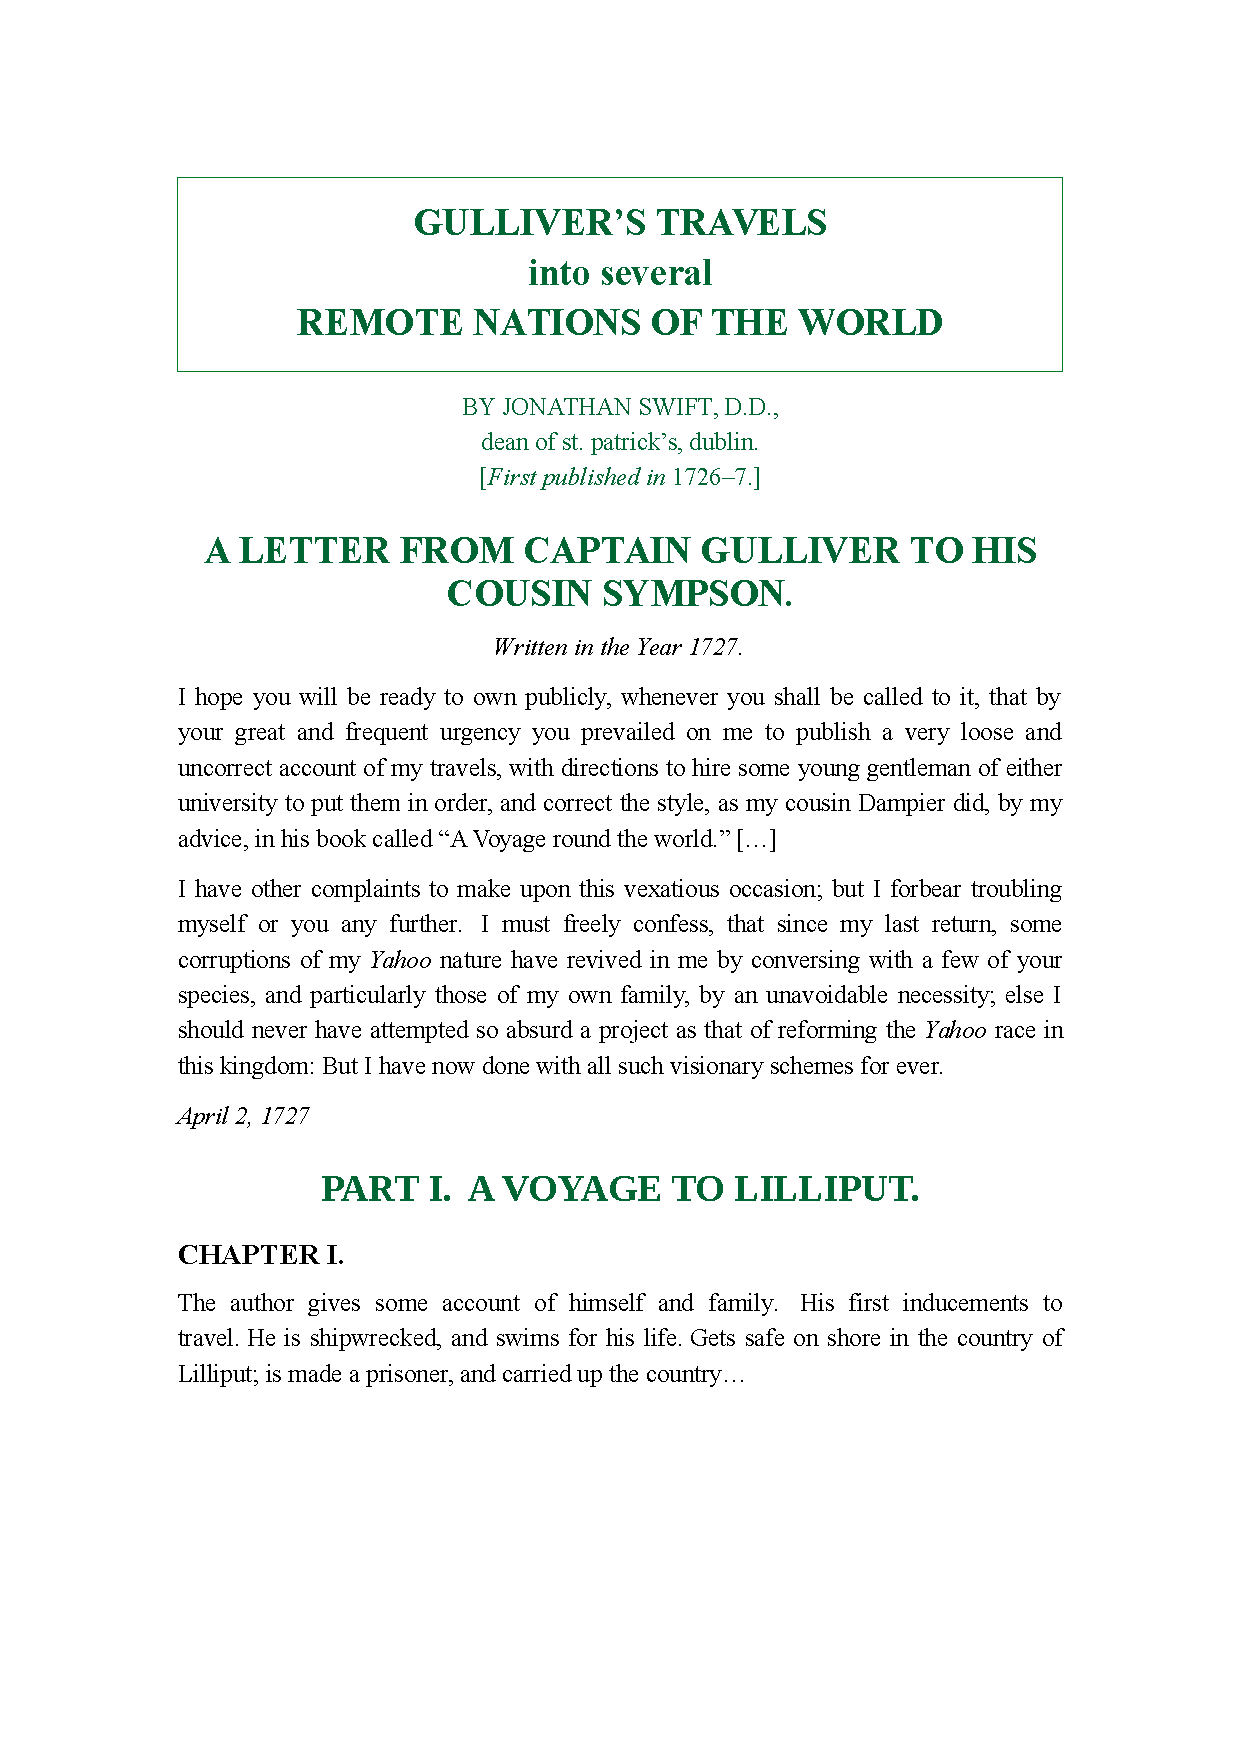
\includegraphics[width=.75\textwidth]{./sources/texte01/ExtraitGulliver6eFormate}}\label{modelePage}\end{center}

\boiteEnonce{Pour parvenir à ce résultat, vous devrez utiliser deux nouvelles fonctionnalités du traitement de texte : passer le texte en majuscule et encadrer un paragraphe. Les opérations à effectuer pour y parvenir sont les suivantes :
\begin{itemize}
\item marges de 3\,cm à gauche, à droite, en haut et en bas ;
\item police de caractères \emph{Times New Roman} ;  
\item titres en caractères de taille 16 points et de couleur \emph{Turquoise} ;
\item texte en caractères de taille 12 points avec un interligne fixe de 0,6\,cm et un espace sous les paragraphes de 0,25\,cm ;
\item quelques parties du texte en italique ; 
\item le texte justifié et les titres centrés.
\end{itemize}}

\boiteEnonce{Une fois la mise en forme terminée, vous devrez exporter votre fichier au format PDF (le fichier doit être nommé à partir de votre nom : \texttt{Nom-date.pdf}) et le rendre sur \emph{Teams} à l'endroit indiqué par votre enseignant.}

\textbf{Pour obtenir de l'aide, rendez-vous à la page \pageref{correction_texte02}}



%
%
%  S  É  A  N  C  E     III
%
%


\section{Séance 3 : mise en forme d'un compte rendu}\label{ficheTexte3}

\prof{cette séance doit être faite sur deux périodes si les élèves préparent eux-mêmes leur compte rendu d'expérience (une période pour la rédaction du compte rendu, et une pour la mise en forme). Il est également possible (comme pour les séances 1 et 2 ci-dessus) de leur donner le compte rendu de la dernière expérience faite, mais non mis en forme, ainsi qu'un modèle de ce qui est attendu. Il faut prévoir une image à insérer dans le compte rendu (format JPG ou PNG), et la mettre à disposition des élèves sur la page \emph{Teams} de votre cours. Précisez aux élèves vos attentes : mise en page, alignements, espacements, taille des caractères, etc.}  

\subsection{L'activité demandée}

\boiteEnonce{Le but de cet exercice est de mettre en forme un compte rendu d'expérience et d'y insérer une image fournie par votre professeur. Vous devez utiliser les techniques apprises dans cette fiche sur le traitement de texte pour préparer votre document.}

\boiteEnonce{Une fois la mise en forme terminée, vous devrez exporter votre fichier au format PDF (le fichier doit être nommé à partir de votre nom : \texttt{Nom-Prénom-date.pdf}) et le rendre sur la plateforme Teams à l'endroit indiqué par votre enseignant.}

\textbf{Pour obtenir de l'aide, rendez-vous à la page \pageref{correction_texte03}}

}







\section{Aide pour réaliser les activités}
\subsection{\label{correction_texte01}Aide pour la Séance 1}

\subsubsection{Mettre en forme la page}\index{Writer!Marges}\index{Marges (Writer)}

Pour commencer on définit la taille des quatre marges du document (gauche, droite, haut et bas). On choisit ici 4\,cm à gauche et à droite, et 3\,cm en haut et en bas.

Dans le menu \texttt{Mise en page}, choisir \texttt{Marges}, puis \texttt{Marges personnalisées...}:    

\uneimageici{./images/texte/forme1.png}{.45\textwidth}

Dans la boîte de dialogue qui s'ouvre, se rendre dans l'onglet \texttt{Marges} puis régler les marges :  

\uneimageici{./images/texte/forme2.png}{.7\textwidth}

Vous pouvez éventuellement vous rendre dans l'onglet \texttt{Mise en page} puis en profiter pour régler les \texttt{En-têtes} et \texttt{Pieds de page}.











\subsubsection{Choisir une police de caractères}\index{Writer!Changer la police de caractères}\index{Police de caractère (Writer)}

Par défaut, la police de caractères du document est \texttt{Calibri} avec une taille de 12. On souhaite passer à \texttt{Times New Roman}. La première étape est de sélectionner tout le texte. Pour cela :

\begin{itemize}
\item soit, on passe par le menu \texttt{Édition} et on choisit \texttt{Sélectionner Tout} ;
\item soit, on utilise le raccourci clavier \texttt{cmd + A}.\index{Raccourci Clavier! Cmd + A, sélectionner tout (Writer)}    
\end{itemize}

\deuximagesici{./images/texte/police1.png}{.7\textwidth}
              {./images/generales/clavierCmdA}{.7\textwidth}

Dans la liste déroulante des polices de caractères (1 dans l'image ci-dessous), choisir la police \texttt{Times New Roman} : le texte sélectionné change alors de police de caractères.  


\uneimageici{./images/texte/police2.png}{.7\textwidth}


\subsubsection{Modifier la taille des caractères}\index{Writer!Taille des caractères}\index{Tailles des caractères (Writer)} 

Avant de modifier la taille des caractères, il faut sélectionner les parties du texte à modifier. On choisit une taille de 12 points pour le texte (on peut utiliser \texttt{cmd + A} pour tout sélectionner ou passer par le menu \texttt{Édition}) et 16 pour le titre (à sélectionner à la souris avant le changement de taille).

\deuximagesici{./images/texte/taille1.png}{.7\textwidth}%
              {./images/texte/taille2.png}{.7\textwidth}







\subsubsection{Centrer du texte}\index{Writer!Centrer le texte}\index{Centrer le texte (Writer)}

Pour centrer les trois premières lignes, il faut tout d'abord les sélectionner à l'aide de la souris. Cliquer ensuite sur le bouton \emph{Centrer le texte} : 

\uneimageici{./images/texte/centrer1.png}{.6\textwidth}

%%%%%%%%%%%%%%%%%%%%%%%%%%%%%%%%%%%%%%%%%%%%%%%%%%%%%%%%%%
%\subsection{Créer une liste à puces}\index{Writer!Liste à puces}\index{Liste à puces (Writer)}   
%
%Les différents personnages de l'acte 1 scène 1 sont présentés sous la forme d'une liste où chaque ligne démarre par un $\bullet$ qui s'appelle une \emph{puce}. L'ensemble est nommé \emph{liste à puces}.   
%
%Pour créer une liste à puce, sélectionner les lignes concernées puis cliquer sur le bouton \emph{Activer les puces}.
%
%\uneimageici{./images/texte/WriterListePuce}{.7\textwidth}
%%%%%%%%%%%%%%%%%%%%%%%%%%%%%%%%%%%%%%%%%%%%%%%%%%%%%%%%%%%




\subsubsection{Souligner du texte}

On souligne le titre.\index{Writer!Souligner}\index{Souligner (Writer)} Pour cela, on le sélectionne, puis on applique une des deux méthodes suivantes :

\begin{itemize}
\item utilisation du bouton \emph{souligner} :  
\uneimageici{./images/texte/souligner1.png}{.7\textwidth}
\item utilisation du raccourci clavier \texttt{cmd + U} :\index{Raccourci Clavier! Cmd + U, souligner (Writer)} 
\uneimageici{./images/generales/clavierCmdU}{.3\textwidth}
\end{itemize}




\subsubsection{Mettre un texte en gras ou en italique}

Pour mettre du texte en gras ou en italique\index{Writer!Gras}\index{Gras (Writer)}\index{Writer!Italique}\index{Italique (Writer)}, il faut tout d'abord le sélectionner, puis appliquer une des deux méthodes suivantes :

% attention, ci-dessous j'ai fait deux listes à puces différentes pour pouvoir conserver 
% une pleine largeur pour les images...
\begin{itemize}
\item utilisation du bouton \emph{gras} ou \emph{italique} :
\end{itemize}
\deuximagesici{./images/texte/gras1.png}{\textwidth}%
              {./images/texte/italique1.png}{\textwidth}
\begin{itemize}
\item utilisation du raccourci clavier \texttt{cmd + B} (gras) ou \texttt{cmd + I} (italique)\index{Raccourci Clavier! Cmd + I, italique (Writer)}\index{Raccourci Clavier! Cmd + B, gras (Writer)} :
\end{itemize}
\deuximagesici{./images/generales/clavierCmdB}{.7\textwidth}%
              {./images/generales/clavierCmdI}{.7\textwidth}


    









\subsubsection{Modifier la couleur des caractères} 


On change la couleur du titre\index{Writer!Changer la couleur des caractères}\index{Couleur des caractères (Writer)}. Pour cela, on le sélectionne, puis on choisit la couleur désirée (par exemple \emph{Rouge foncé}) :

\uneimageici{./images/texte/couleur1.png}{.4\textwidth}










\subsubsection{Mettre en forme des paragraphes}\index{Writer!Interligne}\index{Writer!Espacement entre paragraphes}\index{Interligne (Writer)}\index{Espacement entre paragraphes (Writer)} 



Il faut tout d'abord sélectionner tous les paragraphes sur lesquels on veut appliquer un changement.

Comme l'espace entre les lignes est une propriété du paragraphe, on peut le modifier en passant par le menu \texttt{Mise en forme} puis \texttt{Paragraphe...}

On va modifier deux propriétés : 
\begin{itemize}
\item l'espace entre deux lignes au sein d'un même paragraphe (\emph{interligne}) ;
\item l'espace entre deux paragraphes (\emph{espacement sous le paragraphe}).
\end{itemize}


\uneimageici{./images/texte/paragraphe1.png}{.7\textwidth}

Dans la boîte de dialogue qui s'ouvre, se rendre dans l'onglet \texttt{Retrait et espacement}, puis régler l'interligne et l'espacement sous le paragraphe :  

\uneimageici{./images/texte/paragraphe2.png}{.6\textwidth}







\subsubsection{Justifier un paragraphe}\index{Writer!Justifier}\index{Justifier (Writer)}\index{Aligner le texte à droite et à gauche (justifier) (Writer)}

Lorsque le texte est aligné à la fois du côté gauche et du côté droit, on dit qu'il est \emph{justifié}. Pour justifier les parties du texte qui doivent l'être:

\begin{itemize}
\item sélectionner les paragraphes à justifier à l'aide de la souris
\item cliquer sur le bouton \emph{justifié} ou utiliser le raccourci clavier \texttt{cmd + J}. 
\end{itemize}

\uneimageici{./images/texte/justifier.png}{.7\textwidth}





\subsubsection{Aligner à droite}  

Pour terminer, on aligne à droite les points de suspension finaux. Pour cela, il faut les sélectionner à l'aide de la souris puis cliquer sur le bouton \texttt{Aligner à droite} :  

\uneimageici{./images/texte/alignerDroite.png}{.5\textwidth}



\subsubsection{Exporter au format PDF}\index{Writer!Exporter au format PDF}\index{PDF (exporter au format) (Writer)}

Une fois le travail achevé et sauvegardé, il faut exporter le fichier au format PDF. Pour cela, il faut 
passer par le menu \texttt{Fichier} et choisir \texttt{Enregistrer sous...} à la place de \texttt{Enregistrer}. Il faut ensuite choisir \texttt{Formats d'exportation - PDF}, puis l'emplacement d'enregistrement, comme par exemple \texttt{le Bureau}. Terminez l'exportation en cliquant sur \texttt{Enregister}.

\deuximagesPGici{./images/texte/export1.png}{\textwidth}%
                {./images/texte/export2.png}{\textwidth}



Le fichier PDF est alors enregistré au même endroit que le fichier sur lequel on travaille.


\cadre{Le \textbf{format PDF} est un format parfaitement adapté aux échanges de documents : on ne peut le modifier sans laisser la trace de ce changement, et il est lisible sur tous les périphériques (ordinateurs, tablettes, smartphones) en conservant son aspect initial. Il peut contenir du texte, des images, des liens vers l'internet et même des vidéos ou du son. À chaque fois qu'il faut rendre ou envoyer un document qui n'est pas destiné à être modifié, il faut privilégier le format de fichier PDF.}  








\subsubsection{Remettre le travail achevé sur Teams}

Une fois votre travail terminé et exporté au format PDF, il faut le remettre au professeur. Pour cela, se connecter à la page \emph{Teams} du cours. Chercher le dossier de remise de devoir, puis remettre le travail. Si nécessaire, se reporter à la fiche méthode \emph{Remettre son devoir}, page \pageref{TeamsRemettreDevoir}.  





\subsubsection{Pour aller plus loin...}  

Quand les textes deviennent très longs, il est difficile d'y retrouver un mot en particulier. Les traitements de texte disposent donc d'un outil permettant de rechercher un mot.\index{Writer!Rechercher}\index{Rechercher (Writer)} 

Lorsqu'on souhaite retrouver un mot dans une page de texte, on peut utiliser le raccourci clavier \texttt{cmd + F} :\index{Raccourci Clavier! Cmd + F, rechercher (Writer)}   

\uneimageici{./images/generales/clavierCmdF}{.35\textwidth}

Une barre de recherche s'ouvre alors en haut de la fenêtre :

\uneimageici{./images/texte/WordBarreRecherche.png}{.9\textwidth}

Essayez de rechercher le mot \emph{Belle} : il suffit d'entrer le mot dans la zone de saisie, puis d'appuyer sur la touche \texttt{Entrée}. Pour fermer la barre de recherche, utilisez de nouveau le raccourci clavier \texttt{cmd + F}.   


%%%%%%%%%%%%%%%%%%%%%%%%%%%%%%%%%%%%%%%%%
%\subsubsection{Remplacer les : par des .}\index{Writer!Rechercher et remplacer}\index{Rechercher et remplacer (Writer)}
%
%\uneimageici{./images/texte/WriterEditionMenu}{.35\textwidth}
%
%\uneimageici{./images/texte/WriterBoiteRechercherRemplacer}{.5\textwidth}
%%%%%%%%%%%%%%%%%%%%%%%%%%%%%%%%%%%%%%%%%

\poubelle{

%
%
%  S  É  A  N  C  E     II
%
%


\subsection{Aide pour la Séance 2}\label{correction_texte02}


\subsubsection{Passer le texte en majuscule}\index{Writer!Majuscule}\index{Majuscule (Writer)}

Certaines parties du texte doivent être écrites en majuscules. Pour cela, sélectionner-les\footnote{On peut sélectionner différents endroits du texte en même temps en maintenant la touche \texttt{Cmd} enfoncée pendant qu'on sélectionne les zones à la souris.} puis ouvrir le menu \texttt{Format} et choisir \texttt{Caractère...} Une boîte de dialogue s'ouvre : dans l'onglet \texttt{Effet de caractère}, il faut choisir \texttt{Majuscules}, puis cliquer sur \texttt{OK}.  

\uneimageici{./images/texte/WriterTexteMajuscule}{.9\textwidth}









\subsubsection{Encadrer un paragraphe}\index{Writer!Encadrer}\index{Encadrer (Writer)} 

Pour encadrer le titre de l'ouvrage et ajouter un espacement entre le texte et la bordure qui l'entoure, on utilise l'outil \emph{bordures de paragraphe}. Pour cela, sélectionner le titre, puis ouvrir le menu \texttt{Format} et choisir \texttt{Paragraphe...} Une boîte de dialogue s'ouvre : dans l'onglet \texttt{Bordures}, modifier les propriétés des bordures comme indiqué ci-dessous, puis cliquer sur \texttt{OK}.

\uneimageici{./images/texte/WriterParagrapheEncadre}{.9\textwidth}



\subsubsection{Pour aller plus loin...}

Une fois votre document rendu au format PDF sur la page \emph{Teams} de votre cours, amusez-vous à découvrir toutes les propriétés des paragraphes. Vous pouvez par exemple ajouter :
\begin{itemize}
\item un retrait pour le premier mot du paragraphe ;
\item un retrait pour le paragraphe en entier ; 
\item un arrière plan (une couleur de fond) ;
\item une ombre derrière le paragraphe ; 
\item divers types de bordures. 
\end{itemize}


%
%
%  S  É  A  N  C  E     III
%
%


\subsection{Aide pour la Séance 3}\label{correction_texte03}



\subsubsection{Insérer une image}\index{Writer!Insérer une image}\index{Insérer une image (Writer)}

La première étape est de récupérer sur la page \emph{Teams} du cours l'image à insérer dans le compte rendu. Si nécessaire, se reporter à la fiche méthode \emph{Récupérer un document sur Teams}, paragraphe \vref{MoodlePrendreDoc}.

\vspace{12pt}

Pour insérer une image dans un document texte :

\begin{enumerate}
\item Cliquer sur la souris pour positionner le curseur à l'endroit où l'image doit être insérée et sauter quelques lignes pour laisser de la place à l'image :

\uneimageici{./images/texte/WriterInsertionImage2}{.6\textwidth}

\item Se rendre dans le menu \texttt{Insertion} et choisir \texttt{Image...}

\uneimageici{./images/texte/WriterInsertionImage1}{.6\textwidth}

\item Dans la boîte de dialogue qui s'ouvre, rechercher le fichier qui contient l'image et terminer l'insertion en cliquant sur \texttt{Ouvrir}.

\item L'image peut alors être redimensionnée :
        \begin{itemize}
        \item soit, en utilisant les poignées qui apparaissent lorsqu'on clique sur l'image ;
        \uneimageici{./images/texte/WriterInsertionImage3}{.5\textwidth}
        \item soit, en double-cliquant sur l'image pour faire apparaître la boîte de dialogue suivante. Il faut dans un premier temps cocher la case \texttt{Conserver le ratio}, puis on peut régler les dimensions souhaitées pour l'image.
        \uneimageici{./images/texte/WriterInsertionImage4}{.7\textwidth}
        \end{itemize}
\end{enumerate}


}
%\chapter{Présentation 1}  

Un logiciel de présentation permet de bâtir des diapositives à partir de gabarits de départ qui seront ensuite personnalisés. Ces diapositives s'enrichissent de textes, de vidéos et de mises en forme divrses.

\section*{Synoptique}

{\footnotesize
\begin{itemize}
\item Logiciel \emph{Microsoft PowerPoint} 
\item Matières concernées : titulaire.
\item Compétences : 
        \begin{itemize}
        \item créer une diapositive à partir d'un modèle ; 
	\item créer une diapositive à partir d'une diapositive vide ;
	\item insérer un texte ;
	\item insérer une image ;
	\item insérer une image d'arrière-plan ;
	\item utiliser la trieuse de diapositive ;
	\item utiliser les notes de présentation ;
	\item imprimer les diapositives ;
	\item exporter les diapositives au format \texttt{PDF}.
        \end{itemize}
\item Cette fiche est à réaliser :
        \begin{itemize}
        \item avant les vacances de février. 
        \end{itemize}
\end{itemize}
}% fin du footnotesize


\vfill
\phantom{rien}

%
%
% SEANCE  1
%
%

\pagebreak

\section{Séance 1 : une présentation}\label{fichePresentation6e1}

\subsection{Pour bien démarrer...}

Dès que vous avez ouvert un nouveau document dans \emph{PowerPoint}, sauvegardez-le au format Nom-seance1.pptx : dans le menu \texttt{Fichier}, choisir \texttt{Enregistrer sous}.

\uneimageici{./images/generales/clavierCmdS}{.4\textwidth}


\subsection{Sujet de l'activité...}

\boiteEnonceLarge{Le but de cette séance est créer une présentation sur un thème communiqué par votre enseignant à l'aide du logiciel \emph{Microsoft PowerPoint} et qui utilise tous les points ci-dessous :
\begin{itemize}
	\item une diapositive de titre avec votre nom,
	\item des diapositives de différents styles (texte, image avec texte, image seulement, ...),
	\item des animations entre les diapositives et sur chaque diapositive,
	\item un arrière-plan utilisant une image,
	\item une diapositive de fin avec remerciements,
	\item des notes.
\end{itemize}
\vspace{8pt}
Une fois votre travail terminé, exportez votre présentation au format PDF et enregistrez-le sur votre ordinateur avant de l'envoyer sur \emph{Teams}, à endroit indiqué par votre enseignant.
}% fin énoncé

\textbf{Pour obtenir de l'aide, rendez-vous à la page suivante.}

\subsection{Pour aller plus loin...}

Insérer une vidéo dans votre présentation.



%\vfill

%\cadre{Pensez à sauver régulièrement votre travail en appuyant sur \texttt{Cmd + S} ou à partir du menu \texttt{Fichier} en choisissant \texttt{Enregistrer}.

%\uneimageici{./images/generales/clavierCmdS}{.3\textwidth}



\newpage

\section{Aide pour réaliser l'activité}\label{aidePresentation}

\subsection{Les ingrédients d'une bonne présentation}

Une présentation orale peut s'appuyer sur un diaporama qui permet d'illustrer les propos de l'orateur et lui permet de garder un fil conducteur. Attention, le diaporama est bien une illustration du discours : l'orateur ne doit jamais lire le contenu des diapositives. D'ailleurs les diapositives ne doivent pas contenir de phrase mais seulement des mots-clés, des graphiques, des schémas et des illustrations. Le diaporama ne doit pas entrer en concurrence avec l'orateur, qui doit concentrer l'attention du public.

\subsubsection{Mise en forme du diaporama}

\begin{itemize}
\item Choisir une ligne graphique simple, épurée, identique sur chaque diapositive.
\item Utiliser une police de caractère simple (type Arial ou Times) et de grande taille (par ex. 32 pour les textes et 44 pour les titres). Garder la même police partout.
\item Utiliser des couleurs vives à fort contraste avec le fond (texte foncé sur fond clair). Éviter les textes clairs sur fond noir qui ne se voient pas si la salle n'est pas suffisamment sombre.
\item Numéroter chaque diapositive.
\item Utiliser un minimum d'animations : elles font perdre l'attention de l'auditoire, voire l'agacent.
\item Écrire le minimum de texte : se limiter à quelques mots-clés.
\end{itemize}

\subsubsection{Contenu du diaporama}

\begin{itemize}
\item Première diapositive : titre, prénom, nom, date et une illustration. C'est la diapositive qui est affichée avant même le début de la présentation. L'auditoire doit savoir qui va parler et ce qu'il va présenter.
\item Seconde diapositive : le plan de la présentation.
\item Avant-dernière / dernière diapositive : conclusion et, si nécessaire, remerciements.
\item Entre la diapositive de titre et celle de conclusion, enchaînement logique de diapositives suivant un plan bien défini. Il faut raconter une histoire !
\end{itemize}

\subsubsection{Deux exemples}

Comment présenter l'Institut Florimont ? Ci-dessous, à gauche, une mauvaise diapositive contenant beaucoup de texte. À droite, une diapositive visuellement agréable qui ne contient que les chiffres clés et quelques icônes pour que l'orateur se souvienne de ce qu'il doit dire.

\deuximagesici{./images/presentation/diapoBad}{\textwidth}{./images/presentation/diapoGood}{\textwidth} 



\subsection{Les outils dont vous aurez besoin}\label{Presentation6eOutils}

Les nouveaux outils dont vous aurez besoin pour réaliser les trois séances sur la création d'une présentation sont décrits ci-dessous :


\begin{itemize}   
\item \textbf{créer une nouvelle présentation}, voir section \vref{Presentation1new} ;
\item créer \textbf{une diapositive à partir d'un modèle}, voir section \vref{Presentation1diapoModele} ;
\item utiliser la \textbf{trieuse de diapositives (ordonner, dupliquer et supprimer les diapositives)}, voir section \vref{Presentation1trieuse} ;
\item \textbf{ajouter une diapositive}, voir section \vref{Presentation1nouvelleDiap} ;
\item créer une \textbf{diapositive à partir d'une diapositive vide}, voir section \vref{Presentation1DiapoSansModele} ;
\item \textbf{insérer un texte dans une diapositive}, voir section \vref{Presentation1texte} ;
\item \textbf{insérer une image dans une diapositive}, voir section \vref{Presentation1image} ;
\item \textbf{définir une image d'arrière-plan}, voir section \vref{Presentation1imageFond} ;
\item \textbf{utiliser les animations}, voir section \vref{Presentation1effets} ;

\item \textbf{ajouter des notes de présentations}, voir section \vref{Presentation1notes} ;
\item \textbf{imprimer une présentation et ses notes}, voir section \vref{Presentation1export} ;
\item \textbf{exporter une présentation au format \texttt{PDF}}, voir section \vref{Presentation1exportPDF} 
\end{itemize}  





\subsubsection{Créer une nouvelle présentation}\index{Impress!Créer présentation}\index{Créer présentation (Impress)}\label{Presentation1new}

Ouvrez le navigateur web et allez sur \texttt{office.com}. Cliquez sur le bouton \texttt{Connexion}.

\uneimageici{./images/tableur/ecran_office_com_crop}{.5\textwidth}

Cela ouvre la page de connexion de l'Institut. Entrez votre identifiant et votre mot de passe pour accéder au portail d'office.com. Vous trouverez sur la gauche les boutons menant à toutes les applications d'office. Cliquez sur le logo de \emph{PowePoint}. Cliquez ensuite sur le cadre blanc avec la croix orange pour ouvrir une fenêtre de travail \emph{PowePoint}.

\uneimageici{./images/presentation/ecran_office_PP_crop}{.45\textwidth}





\subsubsection{Une diapositive à partir d'un modèle}\index{Impress!Diapositive à partir modèle}\index{Diapositive à partir modèle (Impress)}\label{Presentation1diapoModele}

Pour créer une diapositive, il faut cliquer sur le bouton \texttt{Nouvelle diapositive}, en haut à gauche de l'espace de travail \circled{1}. S'ouvre alors une liste de modèles, comme présenté ci-dessous. Choisissez le modèle \texttt{Contenu avec légende} en cliquant dessus \circled{2}.

\uneimageici{./images/presentation/Impress_02Creer_01_OPP_crop}{.5\textwidth}



La diapositive est ensuite ajoutée à la présentation.

\uneimageici{./images/presentation/Impress_02Creer_02_OPP_crop}{.6\textwidth}

Ce modèle permet l'insertion très facile de textes et d'images (ou d'autres types de contenu).

% \uneimageici{./images/presentation/Impress_02Creer_02}{.6\textwidth}

\paragraph{Insérer un texte} en cliquant sur le cadre de texte

Cliquez sur le cadre de gauche, dans lequel il est écrit \texttt{Click to add text} (en français : Cliquez pour ajouter du texte). Vous pouvez ensuite immédiatement écrire du texte pour cette partie de la diapositive.

Pour mettre en forme le texte, il faut se rendre à l'onglet Accueil \circled{1}. Les différentes options sont ensuite disponibles en haut de la fenêtre \circled{2}.

\uneimageici{./images/presentation/Impress_02Creer_03_OPP_crop}{\textwidth}




\paragraph{Insérer une image} en cliquant sur l'icône en bas à gauche des options proposées, comme représenté ci-dessous :

\uneimageici{./images/presentation/Impress_03Inserer_01_OPP_crop}{.3\textwidth}

Dans la boîte de dialogue qui s'ouvre, rechercher le fichier qui contient l'image à insérer et terminer en appuyant sur le bouton \texttt{Insérer}.

\vspace{1em}

L'image peut être redimensionnée et tournée :\label{poigneeTourneZoom} 

\begin{itemize}
\item pour \textbf{redimensionner l'image}, cliquer une fois dessus et utiliser les \textbf{poignées} qui apparaissent \circled{1} ;
\item pour effectuer une \textbf{rotation de l'image}, cliquer une fois dessus et utiliser la \textbf{poignée de rotation} qui apparait en haut \circled{2}.
\end{itemize}

\uneimageici{./images/presentation/Impress_03Inserer_02_OPP_crop}{.5\textwidth}

À tout moment il est possible de passer d'un modèle de diapositive à un autre modèle en allant dans l'onglet \texttt{Accueil} \circled{1} puis en cliquant sur \texttt{Disposition} \circled{2}. On remarque alors que l'image et le texte précédemment insérés sont conservés.

\uneimageici{./images/presentation/Impress_03Inserer_03_OPP_crop}{.8\textwidth}



\subsubsection{Trieuse de diapositives (ordonner, dupliquer et supprimer les diapositives)}\index{Impress!Trieuse de diapositive}\index{Trieuse de diapositive (Impress)}\index{Impress!Dupliquer une diapositive}\index{Impress!Ordonner les diapositives}\index{Ordonner les diapositives (Impress)}\index{Impress!Dupliquer une diapositive}\index{Dupliquer une diapositive (Impress)}\index{Impress!Supprimer une diapositive}\index{Supprimer une diapositive (Impress)}\label{Presentation1trieuse}

La trieuse de diapositives est un affichage de l'ensemble de la présentation qui permet de distinguer toutes les diapositives, de naviguer rapidement d'une à l'autre et de les déplacer, de les dupliquer ou encore de les supprimer.

Pour y accéder, il faut choisir l'onglet \texttt{Affichage} \circled{1} puis cliquer sur \texttt{Trieuse de diapositives} \circled{2}.

\uneimageici{./images/presentation/Impress_05Trieuse_01_OPP_crop}{.7\textwidth}

\begin{itemize}
	\item Pour retourner dans la vue normale d'une diapositive, il suffit de double-cliquer dessus ;
	\item Pour déplacer une diapositive, il suffit de cliquer dessus et de maintenir le bouton de souris enfoncé tout en la déplaçant. Relachez le bouton de souris quand la diapositive se trouve où vous le voulez;
	\item Pour dupliquer une diapositive, on peut faire un clic droit dessus et sélectionner \texttt{Dupliquer la diapositive}. ;
	\item Pour supprimer une diapositive, on peut faire un clic droit dessus et sélectionner \texttt{Supprimer la diapositive} ou simplement appuyer sur la touche \texttt{Effacer} (la flèche pointant vers la gauche, au-dessus de la touche \texttt{Entrer}).
\end{itemize}




\subsubsection{Ajouter une diapositive}\index{Impress!Créer diapositive}\index{Diapositive, créer (Impress)}\label{Presentation1nouvelleDiap}

Pour ajouter une diapositive, deux solutions sont possibles :

\begin{itemize}
\item Un clic droit sur une zone vide de la trieuse permet d'insérer une nouvelle diapositive à cet endroit ou de coller une diapositive précédemment copiée à l'aide de \texttt{Cmd + C} (figure à gauche) ; 
\item un clic droit sur une diapositive dans la trieuse permet de choisir d'appliquer les options précédentes comme si on avait cliqué juste après cette diapositive ou de dupliquer la diapositive sélectionnée (figure ci-dessous à droite).
\end{itemize}
	
\deuximagesici{./images/presentation/Impress_04NouvelleDia_02_OPP_crop}{.7\textwidth}
	      {./images/presentation/Impress_04NouvelleDia_03_OPP_crop}{.7\textwidth}



\subsubsection{Diapositive à partir d'une diapositive vide}\index{Impress!Diapositive sans modèle}\index{Diapositive à partir d'une diapositive vide (Impress)}\label{Presentation1DiapoSansModele}


%\begin{minipage}[c]{.58\textwidth}
Si aucun des modèles proposés ne convient à ce que l'on souhaite réaliser, on peut partir d'une diapositive vide. Par exemple, la diapositive montrée sur la figure ci-dessous est réalisée à partir d'une diapositive vide plutôt qu'à partir d'un modèle.

%\centering%
%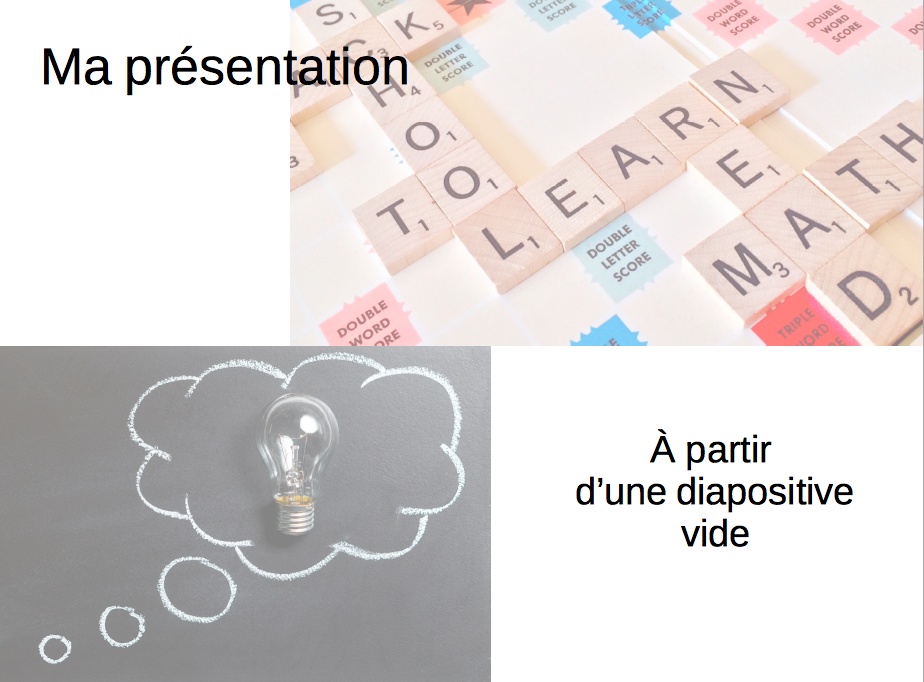
\includegraphics[angle=0,width=.75\textwidth]{./images/presentation/Impress_07DiaSansFormat_10}
\uneimageici{./images/presentation/Impress_07DiaSansFormat_10}{.4\textwidth}

%\end{minipage}\hfill%

\subsubsection{Insérer un texte dans une diapositive}\index{Impress!Insérer un texte}\index{Texte, insérer (Impress)}\label{Presentation1texte}
%\begin{minipage}[c]{.38\textwidth}

%\end{minipage}

\vspace{1em}

La première étape est de sélectionner une diapositive vide dans le choix de modèles comme montré dans la figure ci-dessous.



\uneimageici{./images/presentation/Impress_07DiaSansFormat_02_OPP_crop}{.7\textwidth}

Pour ajouter du texte sur cette diapositive, il faut se rendre sous l'onglet \texttt{Insertion} \circled{1} et utiliser l'outil \texttt{Zone de texte} \circled{2}.

\uneimageici{./images/presentation/Impress_07DiaSansFormat_03_OPP_crop}{.8\textwidth}

Une fois la zone de texte posée, on peut immédiatement commencer à écrire dedans. Les options de mise en forme du texte se retrouvent dans l'onglet \texttt{Accueil} \circled{1}. Les poignées de saisie et de rotation permettent de modifier la taille et l'orientation de la zone de texte, comme s'il s'agissait d'une image \circled{2}.

\uneimageici{./images/presentation/Impress_07DiaSansFormat_04_OPP_crop}{.7\textwidth}

\vspace{1em}

En cliquant sur le cadre de l'espace de texte (mais pas sur les poignées de saisie), on peut ensuite le déplacer sur la diapositive. 

\vspace{1em}

Pour modifier la taille des caractères, deux possibilités :
\begin{itemize}
\item sélectionner toute la zone de texte en cliquant sur le cadre (\circled{1} sur la figure ci-dessous à gauche) puis choisir la taille des caractères (\circled{2}) ; 
\item sélectionner le texte uniquement (figure à droite ci-dessous), puis choisir la taille des caractères.
\end{itemize}

\deuximagesici{./images/presentation/Impress_07DiaSansFormat_03_OPP2_crop}{.9\textwidth}
	      {./images/presentation/Impress_07DiaSansFormat_04_OPP2_crop}{.9\textwidth}


\subsubsection{Insérer une image dans une diapositive}\index{Impress!Insérer une image}\index{Image, insérer (Impress)}\label{Presentation1image}

Pour insérer une image, il faut se rendre dans l'onglet \texttt{Accueil} \circled{1}, puis cliquer sur le bouton \texttt{Image} \circled{2}, ce qui ouvre une liste de sources possibles pour l'image. Choisir \texttt{Cet appareil...} \circled{3} pour importer directement une image enregistrée sur l'ordinateur. Les autres options permettent de choisir des images autre part.

\uneimageici{./images/presentation/Impress_07DiaSansFormat_08_OPP_crop}{.7\textwidth}



\subsubsection{Définir une image d'arrière-plan}\index{Impress!Image d'arrière-plan}\index{Image d'arrière-plan (Impress)}\label{Presentation1imageFond}

Pour ajouter une image en arrière-plan de la diapositive, c'est-à-dire une image qui occupe tout le fond de la diapositive, il faut accéder au menu de mise en forme de l'arrière-plan. Pour cela, sous l'onglet \texttt{Création} \circled{1}, cliquer sur \texttt{Mise en forme de l'arrière-plan} \circled{2}. Le \texttt{Remplissage uni} \circled{3} permet de choisir une couleur à utiliser comme fond, et l'option \texttt{Image à partir d'un fichier} \circled{4} permet d'importer une image qui sera utilisée comme arrière-plan.

\uneimageici{./images/presentation/imageAPmenu_OPP_crop}{.7\textwidth}


Pour supprimer une image d'arrière-plan (ou tout autre arrière-plan personnalisé), il faut se rendre dans le même menu de mise en forme d'arrière-plan et cliquer sur \texttt{Arrière-plan uni} et choisir le blanc : la diapositive aura à nouveau un arrière-plan blanc uni. 



\subsubsection{Utiliser les animations}\index{Impress!Animations}\index{Animation (Impress)}\label{Presentation1effets}

Les animations permettent par exemple de faire afficher une diapositive en plusieurs temps : certaines parties de la diapositive arrivant après d'autres ou disparaissant avant le reste de la diapositive. Mais attention, il faut faire un usage parcimonieux des animations : les diaporamas en contenant trop sont souvent pénibles à suivre !

La première étape pour ajouter une animation est de sélectionner l'élément de la diapositive devant être affiché après les autres, comme par exemple un texte \circled{1}. Ensuite, il faut se rendre dans l'onglet \texttt{Animations} \circled{2} et choisir l'animation que l'on souhaite utiliser. Il existe plusieurs types d'animations, comme les effets d'entrée \circled{3}, les effets d'accentuation \circled{4} ou les effets de sortie \circled{5}. Pour une animation de texte arrivant sur la diapositive, c'est un effet d'entrée qu'il faut choisir.

\uneimageici{./images/presentation/Impress_08_Transitions_01_OPP_crop}{.6\textwidth}

Si une diapositive doit contenir plus d'une animation, il faut décider dans quel ordre elles ont lieu. Par exemple, un texte doit apparaitre avant une image, et on veut ensuite retirer l'image pour ajouter encore plus de texte. Pour réaliser ce genre de séquence, il faut d'abord voir comment les animations sont ordonnées : grâce à une numérotation apparaissant dans des rectangles à côté des éléments affectés \circled{1}. En sélectionnant un de ces éléments, on peut cliquer sur les boutons \texttt{Déplacer avant} et \texttt{Déplacer après} \circled{2} pour avancer ou reculer cette animation dans la liste.

\uneimageici{./images/presentation/Impress_08_Transitions_02_OPP_crop}{.6\textwidth}

Pour supprimer une animation, il faut sélectionner l'élément de la présentation qui a une présentation que l'on désire retirer et choisir \texttt{Aucune}.


Si on veut voir les animations des diapositives, on peut lancer le diaporama. Pour faire cela, il faut utiliser l'un des deux boutons suivants:
\begin{itemize}
	\item Le petit bouton Diaporama, en bas à droite, lance le diaporama à partir de la diapositive à l'écran. \circled{1}
	\item Dans l'onglet \texttt{Diaporama} \circled{2}, le bouton \texttt{À partir de la diapositive actuelle} permet également de lancer le diaporama à partir de ce pointr. \circled{3}
	\item Dans le même onglet, le bouton \texttt{À partir du début} permet de lancer le diaporama depuis le début. \circled{4}
\end{itemize}

\uneimageici{./images/presentation/Impress_08_Transitions_04_OPP_crop}{\textwidth}

En mode diaporama, il existe de nombreux moyens de naviguer entre les diapositives:
\begin{itemize}
	\item Les touches de déplacement $\leftarrow$, $\uparrow$, $\rightarrow$ et $\downarrow$ ;
	\item La touche espace ;
	\item Les touches n (comme "next", suivant) et p (comme "previous", précédent) ;
	\item Un clic de souris ;
	\item Le menu d'options se révélant en bas à gauche de la présentation. Il permet notamment d'atteindre directement une diapositive spécifique.	\circled{5}
\end{itemize}

Enfin, on peut quitter un diaporama avant d'être arrivé au bout grâce à la touche Esc.


\subsubsection{Ajouter des notes de présentation}\index{Impress!Notes de présentation}\index{Notes de présentation (Impress)}\label{Presentation1notes}


%\begin{minipage}[c]{.68\textwidth}
Il est possible d'ajouter des \emph{\og notes \fg} associées aux diapositives. Ces notes servent d'aide au présentateur et n'apparaissent pas à l'écran lors de la présentation (sauf sur l'écran secondaire s'il y en a un).

Pour ajouter des notes à une diapositive, sélectionner la diapositive à laquelle on veut les ajouter et cliquer sur le bouton \texttt{Notes}, en bas de l'écran.

\uneimageici{./images/presentation/Impress_06Notes_01_OPP_crop}{.4\textwidth}

Apparait alors en bas de l'écran un espace de texte dans lequel vous pouvez rédiger vos notes.

\uneimageici{./images/presentation/Impress_06Notes_02_OPP_crop}{.7\textwidth}


\subsubsection{Imprimer une présentation et ses notes}\index{Impress!Imprimer}\index{Imprimer (Impress)}\label{Presentation1export}

Pour imprimer les diapositives et les notes associées, il faut se rendre dans le menu \texttt{Fichier} et choisir \texttt{Imprimer...}. \circled{1} Il faut ensuite choisir ce qu'on désire imprimer.

\begin{itemize}
	\item La première option imprime une diapositive par page \circled{2} ;
	\item La deuxième fait de même mais ajoute les notes aux côtés des diapositives \circled{3} ;
	\item La dernière imprime trois diapositives par page avec de la place pour y écrire des commentaires. \circled{4}
\end{itemize}

\uneimageici{./images/presentation/Impress1_impression01_OPP_crop}{.5\textwidth}

Quelle que soit l'option sélectionnée, un fichier PDF contenant ce qui doit être imprimé est préparé. Il suffit de l'ouvrir avant de pouvoir l'imprimer normalement. Pour ce faire, cliquer sur les touches \texttt{Cmd + P} pour ouvrir la fenêtre d'impression. Là, on peut choisir le nombre de copies, l'organisation des pages, et toutes les autres options d'impression. Pour lancer l'impression, cliquer sur le bouton \texttt{Imprimer}, en bas à droite de la fenêtre.

\uneimageici{./images/presentation/Impress1_impression02_OPP_crop}{.5\textwidth}


\subsubsection{Exporter une présentation et ses notes au format PDF}\index{Impress!Exporter au format PDF}\index{Exporter au format PDF (Impress)}\label{Presentation1exportPDF}


Pour exporter une présentation au format PDF, il faut procéder comme indiqué plus haut, mais à la fenêtre d'impression, au lieu de cliquer sur \texttt{Imprimer}, il faut choisir le bouton \texttt{PDF}, en bas à gauche. On peut alors enregistrer le fichier PDF contenant la présentation.

\uneimageici{./images/presentation/Impress1_impression03_OPP_crop}{.45\textwidth}


\vfill
\phantom{rien}







%\chapter{Traitement d'images}\label{ficheImage1}  

Un logiciel de traitement d'images est un logiciel qui permet de retoucher une image existante : taille de l'image, luminosité, contraste, recadrage, etc...\\

\prof{on pourra ici indiquer qu'il existe plusieurs logiciels de traitement d'images, l'un des plus connus étant Photoshop d'Adobe. Le logiciel de traitement d'images utilisé ici est Gimp. Il présente l'avantage d'être libre et gratuit. L'utilisation de nombreuses fonctions est la même pour ces deux logiciels.}

{\footnotesize
\begin{itemize}
\item Logiciel\footnote{Le logiciel Gimp est librement téléchargeable : \url{http://www.gimp.org/}} : \emph{Gimp}
\item Prérequis : aucun
\item Matières concernées : arts visuels et histoire-géographie
\item Objectifs : utiliser un logiciel de retouche d'image pour effectuer des modifications sur une image existante puis l'exporter au format JPG ou PNG (documents à rendre sur Teams).
\item Compétences : 
        \begin{itemize}
        \item format d'image JPG et PNG ;
        \item capture d'écran ;
        \item recadrage.
        \end{itemize}
\item Cette fiche est à réaliser :
        \begin{itemize}
        \item avant la fin du semestre de cours en arts visuels ;
        \item après la séance 1 en français  ;
        \item avant la fin du semestre de cours en arts visuels. 
        \end{itemize}
\prof{\item vous devez préparer trois éléments \underline{avant} la séance : \begin{itemize}\item récupérer sur Teams le fichier \texttt{photoFlorimont.png} qui contient une image aérienne de Florimont, sur laquelle les élèves travailleront ;\item mettre à disposition des élèves sur la page Teams de votre cours le fichier \texttt{ExtraitMoliere6e.odt} \item créer un dossier de remise de devoir sur la page Teams de votre classe car les élèves rendent cette activité sous la forme d'un fichier PDF déposé sur Teams.\end{itemize}}
\end{itemize}
}




\newpage

\section{Séance 1 : recadrer une image}\index{Gimp!Recadrer une image}\index{Recadrage d'une image (Gimp)}

\subsection{Premiers pas avec Gimp }\index{Ouvrir!Gimp}\index{Gimp!Ouvrir}

\prof{par défaut le logiciel Gimp s'ouvre en mode multi-fenêtres, et avec la boîte à outils non activée. Après l'ouverture du logiciel, il faut veiller à ce que tous les élèves aient une interface similaire à celle montrée ci-dessous. Si les différents boîte à outils ne sont pas tout à fait au même endroit, ce n'est pas grave. En effet, l'ordre dans lequel on effectue les opérations détermine la position finale des boîtes d'outils.}

Lancer le logiciel en utilisant la <<\,loupe\,>> :

\uneimageici{./images/generales/loupe}{.7\textwidth}

... puis en indiquant \emph{Gimp} :

\uneimageici{./images/generales/loupeRechercheGimp}{.7\textwidth}


La fenêtre principale du logiciel s'ouvre :

\uneimageici{./images/gimp/GimpInterface}{.7\textwidth}

Si elle ne ressemble pas à celle-ci, alors il faut effectuer les réglages suivants :

\begin{minipage}[c]{.58\textwidth}
\begin{itemize}
\item Ouvrir le menu \texttt{Fenêtre}, puis cocher la case \texttt{Mode fenêtre unique}.
\item Dans le même menu, cliquer également sur \texttt{Boîte à outils} pour faire apparaître les outils.
\end{itemize}
\end{minipage}\hfill%
\begin{minipage}[c]{.38\textwidth}
\uneimageici{./images/gimp/GimpMenuFenetre2}{.9\textwidth}
\end{minipage}




%
%
%  S  É  A  N  C  E     I
%
%






\subsection{Pour bien démarrer...}

Sur la page Teams de votre cours, récupérer le fichier \texttt{photoFlorimont.png}. Si nécessaire, se reporter à la fiche méthode \emph{Consulter le sujet d'un devoir en pièce jointe}, page \pageref{consulterDevoir}.

Une fois le fichier enregistré sur le \emph{Bureau} de l'ordinateur, revenir dans \emph{Gimp}, cliquer sur le menu \texttt{Fichier}, puis \texttt{Ouvrir}.

\uneimageici{./images/gimp/GimpOuvrirFichier}{.4\textwidth}

Chercher dans la zone \emph{Raccourcis} le \emph{Bureau} : le fichier à ouvrir peut alors être sélectionné dans la zone centrale de la boîte de dialogue :

\uneimageici{./images/gimp/GimpOuvrirFichier2}{.6\textwidth}

Achever l'ouverture en cliquant sur le bouton \texttt{Ouvrir}.

\subsubsection{Pensez à enregistrer régulièrement}

Dès que vous avez ouvert un nouveau document dans \emph{Gimp}, sauvegardez-le au format Nom-date.jpg : dans le menu \texttt{Fichier}, choisir \texttt{Enregistrer}. Pendant que vous travaillez, pensez à sauvegarder régulièrement votre travail (raccourci clavier \texttt{Cmd + s}).   

\uneimageici{./images/generales/clavierCmdS}{.4\textwidth}

%\vfill
%\phantom{rien}


\subsection{L'activité demandée}

\vspace{10pt}

\prof{Assurez-vous que tous les élèves ont franchi les premières étapes ci-dessus. Lire ensuite l'énoncé avec les élèves et montrer le résultat attendu (affichage au TBI du résultat). Expliquez bien où trouver le fichier de départ. À partir de ce point, les élèves travaillent chacun à leur rythme.}

\boiteEnonce{Dans cette activité, vous allez recadrer une photographie aérienne de Florimont, dont vous venez de récupérer une version <<\,brute\,>> au format PNG. L'objectif est d'obtenir le résultat suivant :
\begin{center}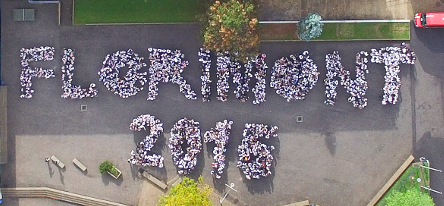
\includegraphics[width=.7\textwidth]{./images/gimp/photoFlorimontReduite}\label{modeleImage}\end{center}
Une fois le cadrage terminé, vous devrez exporter votre fichier au format JPG. Le fichier sera nommé à partir de votre nom : \texttt{Nom-date.jpg} et sera rendu sur Teams à l'endroit indiqué par votre enseignant. Si nécessaire, se reporter à la fiche méthode \emph{Remettre son devoir}, page \pageref{TeamsRemettreDevoir}}



\textbf{Pour obtenir de l'aide, rendez-vous à la page \pageref{correction_gimp01}}

\subsection{Pour aller plus loin...}

Si vous avez terminé votre travail, entraînez-vous à réaliser des captures d'écran (voir page \pageref{CaptureEcran}).










\newpage





%
%
%  S  É  A  N  C  E     II
%
%



\section{Séance 2 : recadrer et encadrer une image}\label{ficheImage2}\index{Gimp!Ajouter un cadre autour d'une image}\index{Cadre autour d'une image (Gimp)}

\prof{cette séance a lieu après la séance \no 1 et réutilise les mêmes outils. Vous devez préparer avant la séance une image de votre choix (au format PNG) qui soit en lien avec votre cours du moment (remarque : cette image doit être compatible avec l'ajout d'un cadre de 1\,cm autour (voir la partie qui traite de l'ajout d'un cadre). Cette image doit être mise à disposition des élèves sur la page Teams de votre cours. Demander ensuite aux élèves d'effectuer le recadrage suivant les consignes données ci-dessous. L'image finale, au format JPG, sera récupérée sur Teams (il faut donc préparer un dossier de remise de devoirs).}  

\subsection{Pour bien démarrer...}

Dès que vous avez ouvert un nouveau document dans \emph{Gimp}, sauvegardez-le au format Nom-date.jpg : dans le menu \texttt{Fichier}, choisir \texttt{Enregistrer}. Pendant que vous travaillez, pensez à sauvegarder régulièrement votre travail (raccourci clavier \texttt{Cmd + s}).   

\uneimageici{./images/generales/clavierCmdS}{.4\textwidth}

\subsection{L'activité demandée}

\vspace{10pt}

\boiteEnonce{Dans cette activité, vous allez recadrer une image mise à votre disposition par votre professeur sur la page Teams de votre cours, en respectant les consignes qui vous seront données, puis vous aller ajouter un cadre blanc autour de cette image. Cette image, dont vous venez de récupérer une version <<\,brute\,>>, est au format PNG.\newline \\
Une fois l'encadrement terminé, vous devrez exporter votre fichier au format JPG.. Le fichier sera nommé à partir de votre nom : \texttt{Nom-date.jpg}) et sera rendu sur la Teams à l'endroit indiqué par votre enseigant. Si nécessaire, se reporter à la fiche méthode \emph{Remettre son devoir}, page \pageref{TeamsRemettreDevoir}}





\subsection{Pour aller plus loin...}

Si vous avez terminé votre travail, entraînez-vous à réaliser des captures d'écran (voir page \pageref{CaptureEcran}).


\newpage

%
%
%  S  É  A  N  C  E     III
%
%


\section{Séance 3 : recadrer et régler luminosité, contraste}\label{ficheImage3}

\prof{faire réfléchir les élèves sur les différents types de cadrage et l'équilibre d'une composition. Les élèves sont ici libres de choisir leur cadrage ; vous pouvez donc les aiguiller vers un cadrage classique, personnel, ou plus créatif. \underline{Avant la séance}, vous devez déposer l'image brute sur la page Teams de votre cours, et préparer un dossier de remise de devoir. L'image brute pour cette activité est disponible sur Teams.}

\subsection{Pour bien démarrer...}

Dès que vous avez ouvert un nouveau document dans \emph{Gimp}, sauvegardez-le au format Nom-date.jpg : dans le menu \texttt{Fichier}, choisir \texttt{Enregistrer}. Pendant que vous travaillez, pensez à sauvegarder régulièrement votre travail (raccourci clavier \texttt{Cmd + s}).   

\uneimageici{./images/generales/clavierCmdS}{.4\textwidth}

\subsection{L'activité demandée}

\vspace{10pt}

\boiteEnonce{Le but de cet exercice est de retoucher une image représentant un détail des vitraux de la chapelle de l'école dont vous devez récupérer une version <<\,brute\,>> au format PNG sur la page Teams de votre cours. Vous devrez :
\begin{itemize}
\item choisir un cadrage en fonction des consignes données par votre professeur ;
\item régler la luminosité et le contraste selon les indications du paragraphe \vref{GimpLumiContraste} ;
\item ajouter un cadre autour de l'image. 
\end{itemize}\vspace{0.5cm}
L'image brute à modifier est la suivante :
\uneimageici{./images/gimp/vitrauxSmall}{.3\textwidth}
Une fois votre travail terminé, vous devrez exporter votre fichier au format JPG (le fichier doit être nommé à partir de votre nom : \texttt{Nom-date.jpg}) et le rendre sur Teams, à l'endroit indiqué par votre professeur. Si nécessaire, se reporter à la fiche méthode \emph{Remettre son devoir}, page \pageref{TeamsRemettreDevoir}}









\subsection{Pour aller plus loin : réaliser une copie d'écran}\label{CaptureEcran}\index{Capture d'écran}\index{Gimp!Capture d'écran}

Il est parfois nécessaire de copier le contenu de l'écran sous forme d'image pour pouvoir l'utiliser dans un document ou une présentation.

\vspace{12pt}

Pour réaliser une copie d'écran :

\begin{enumerate}
\item Capturer l'écran en utilisant un des raccourcis clavier suivant :
        \begin{itemize}
        \item \texttt{Ctrl + Maj + Cmd + 3} pour copier la totalité de l'écran,\index{Raccourci Clavier! Ctrl + Maj + Cmd + 3, copier tout l'écran}
        \item \texttt{Ctrl + Maj + Cmd + 4} pour copier une partie de l'écran (à sélectionner à la souris) ;\index{Raccourci Clavier! Ctrl + Maj + Cmd + 4, copier une partie de l'écran}
        \end{itemize} 

\uneimageici{./images/generales/clavierCapEcran}{.6\textwidth}

\item Coller l'image dans un nouveau document sous \emph{Gimp} : 
\end{enumerate}

\uneimageici{./images/gimp/GimpCollerCommeImage}{.6\textwidth}

On peut alors retravailler l'image comme vous l'avez appris dans cette fiche sur \emph{Gimp}. 





\newpage

\section{Aide pour réaliser les activités}

\subsection{Aide pour la séance 1}


\subsubsection{Utiliser l'outil de découpage}\index{Gimp!Découpage d'une image}\index{Découpage d'une image (Gimp)}\label{correction_gimp01}

Pour découper une partie de l'image afin d'effectuer un recadrage, il faut utiliser l'outil de découpage (icône 
\includegraphics[width=.04\textwidth]{./images/gimp/cutter}) présent dans la boîte à outils.

Sélectionner à l'aide de la souris la zone de l'image à conserver : pour cela, cliquer sur l'image, puis, en maintenant le bouton enfoncé, faire glisser la souris jusqu'à un autre point de l'image. 

\uneimageici{./images/gimp/GimpDecouper1}{.8\textwidth}

La zone sélectionnée est modifiable en déplaçant les 4 angles du rectangle sélectionné. Une fois le cadrage fait, appuyer sur la touche \texttt{Entrée} pour terminer.


\subsubsection{Sauvegarder le fichier}

Il est important de sauvegarder régulièrement le fichier sur lequel on travaille.

Pour enregistrer votre travail :
\begin{itemize}
\item Ouvrir le menu \texttt{Fichier}.
\item Choisir \texttt{Enregistrer sous...}
\item Choisir comme emplacement le \emph{Bureau} de l'ordinateur.
\item Entrer le nom du fichier sous la forme \texttt{Nom-Prénom-date.xcf} \emph{(remarque : XCF est le format de fichier du logiciel Gimp)} 
\item Terminer en cliquant sur \texttt{Enregistrer}.   
\end{itemize}

\uneimageici{./images/gimp/GimpEnregistrerFichier}{.6\textwidth}

Après ce premier enregistrement, pensez à appuyer régulièrement sur la combinaison de touche \texttt{cmd} + \texttt{S} : c'est le \emph{raccourci clavier} permettant d'enregistrer le fichier sur lequel vous êtes en train de travailler.

\uneimageici{./images/generales/clavierCmdS}{.5\textwidth}



\cadre{\textbf{Différence entre \texttt{Enregistrer} et \texttt{Enregistrer sous...}}\newline Dans la plupart des logiciels, on peut : \begin{itemize}\item \textbf{enregistrer} le fichier sur lequel on travaille. Cette opération est possible si le fichier existe déjà et possède un nom. La version courante du fichier sera alors écrite en mémoire et remplacera l'ancienne version du fichier.\item \textbf{enregistrer sous...} le fichier sur lequel on travaille. Cette opération commence par demander un nouveau nom pour l'enregistrement du fichier. On peut donc ouvrir un fichier que l'on ne souhaite pas modifier, choisir \emph{enregistrer sous}, donner un nouveau nom et ainsi travailler sur une copie du fichier de départ.\item utiliser \texttt{cmd + S} (\emph{S} pour \emph{Save}) pour \textbf{enregistrer} le fichier courant. Bien que les documents soient enregistrés automatiquement par la majorité des logiciels, il faut régulièrement sauver son travail pour éviter les surprises.\end{itemize}}






\subsubsection{Exporter l'image dans un autre format}

Il existe de nombreuses manières de coder une image dans un ordinateur. On parle de \emph{format d'image}. Les plus connus et utilisés sont les formats JPG, TIF, PNG et SVG. Ils ont chacun leurs propres caractéristiques, avantages et inconvénients. Dans \emph{Gimp}, les menus \texttt{Enregistrer} et \texttt{Enregistrer sous...} ne permettent que d'enregistrer les images au format XCF. Ce format XCF n'est par contre lisible que par le logiciel \emph{Gimp} ; il faut donc convertir l'image vers un autre format pour qu'elle soit lisible partout. Pour convertir l'image dans un autre format, il faut procéder de la manière suivante : 

\begin{itemize}
\item Ouvrir le menu \texttt{Fichier}.
\item Choisir \texttt{Export As...}
\item Choisir comme emplacement le \emph{Bureau} de l'ordinateur.
\item Comme votre fichier s'appelle déjà \texttt{Nom-Prénom-date.xcf}, \emph{Gimp} propose par défaut comme nom de fichier exporté : \texttt{Nom-Prénom-date.png}. Modifier l'extension du nom de fichier : effacer le \texttt{png} proposé par défaut et le remplacer par \texttt{jpg}.
\item Cliquer sur \texttt{Exporter}.
\item Une deuxième boîte de dialogue s'affiche dans laquelle on peut régler certains paramètres pour la qualité de l'image exportée. On peut garder les valeurs par défaut et cliquer directement sur \texttt{Exporter}.
\end{itemize}
\deuximagesGPici{./images/gimp/GimpExportAs1}{\textwidth}%
		      {./images/gimp/GimpExportAs2}{.8\textwidth}

% SEANCE 2
\subsection{Aide pour la séance 2}


\subsubsection{Ajouter un cadre autour de l'image}\label{GimpCadre}

Pour ajouter un cadre autour de l'image, il faut ajouter de l'espace autour de celle-ci. Cela se fait en modifiant le \emph{canevas} qui est le support de l'image. Quand on agrandit le canevas, on crée un espace vide autour de l'image. Lorsqu'on exportera l'image au format JPG, cet espace sera rempli de blanc.


\begin{minipage}[c]{.38\textwidth}
\begin{itemize}
\item Ouvrir le menu \texttt{Image}.
\item Choisir\\ \texttt{Taille du canevas...}
\end{itemize}
\end{minipage}\hfill%
\begin{minipage}[c]{.58\textwidth}
\uneimageici{./images/gimp/GimpTailleCanevas1}{\textwidth}
\end{minipage}

\begin{minipage}[c]{.38\textwidth}
\begin{itemize}
\item La boîte de dialogue qui s'ouvre indique la taille de l'image en pixels (\texttt{px}).
\end{itemize}
\end{minipage}\hfill%
\begin{minipage}[c]{.58\textwidth}
\uneimageici{./images/gimp/GimpTailleCanevas2}{\textwidth}
\end{minipage}

\begin{itemize}
\item Cliquer sur la case indiquant l'unité (\emph{px}) et choisir \emph{centimètres}.
\item Ajouter 1\,cm à la largeur et à la longueur déjà indiquées.
\item Cliquer sur le bouton \texttt{centrer} pour que l'image soit centrée sur le nouveau canevas plus grand.
\item Cliquer sur \texttt{Redimensionner} pour terminer.
\end{itemize}

\uneimageici{./images/gimp/GimpTailleCanevas3}{.65\textwidth}

La bordure ajoutée autour de l'image est transparente et est représentée par un damier :
\uneimageici{./images/gimp/GimpTailleCanevas4}{.6\textwidth}

Après export au format JPG, on peut constater que la bordure de l'image apparaît bien en blanc.



% SEANCE 3
\subsection{Aide pour la séance 3}


\subsubsection{Luminosité et contraste}\label{GimpLumiContraste}\index{Gimp!Luminosité}\index{Luminosité (Gimp)}\index{Gimp!Contraste}\index{Contraste (Gimp)}


La \textbf{luminosité} d'une image correspond à sa clarté : plus la luminosité est élevée, plus l'image est claire. Plus la luminosité est faible, plus l'image est sombre.

\vspace{12pt}

Le \textbf{contraste} correspond aux différences de luminosité au sein d'une image : plus le contraste est élevé, plus les différences entre les parties lumineuses et les parties sombres de l'image sont marquées.

\vspace{12pt}

Pour régler la luminosité et le contraste d'une image, il faut se rendre dans le menu \texttt{Couleurs} et choisir \texttt{Luminosité-Contraste...} :

\uneimageici{./images/gimp/GimpLuminositeContraste1}{.6\textwidth}

Dans la boîte de dialogue qui s'ouvre, deux curseurs sont disponibles. En bougeant leur position, on peut régler la luminosité ou le contraste de l'image. Les modifications effectuées sont directement visibles à l'écran. Une fois le réglage effectué, cliquer sur le bouton \texttt{Valider} pour terminer.  

\uneimageici{./images/gimp/GimpLuminositeContraste2}{.6\textwidth}




%\newpage





%
%
%  S  É  A  N  C  E     I
%
%



\section{Aide pour réaliser les activités}

\subsection{Aide pour la séance 1}\label{correction_scratch1}




Nous allons écrire le programme étape par étape.


\subsubsection{Modifier la scène où se passe l'action}\index{Scratch!Modifier la scène}\index{Modifier la scène (Scratch)}

La scène correspond à l'arrière-plan (blanc au départ) où se passe l'action. La scène est un objet qui peut être modifié. Pour cela, la première étape est de cliquer sur l'icône scène 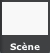
\includegraphics[width=1cm]{./images/scratch/Scene} en bas à droite.

\uneimageici{./images/scratch/ScratchSelectionScene}{.65\textwidth}

Une fois la scène sélectionnée (elle est alors entourée en couleur), suivre les 4 étapes suivantes :

\begin{enumerate}
\item Cliquer sur l'onglet \texttt{Arrière-plans}.
\item Cliquer sur le bouton \texttt{Importer}.
\item Choisir l'arrière-plan \texttt{xy-grid}.
\item Cliquer alors sur le bouton \texttt{OK}. 
\end{enumerate}


\uneimageici{./images/scratch/ScratchChangerScene1}{.8\textwidth}

Notre programme comporte maintenant deux scènes différentes : \texttt{arrière-plan1} et \texttt{xy-grid}. C'est cette dernière qui est sélectionnée (elle est entourée en couleur).

\uneimageici{./images/scratch/ScratchChangerScene2}{.4\textwidth}






\subsubsection{Enregistrer le programme}\index{Enregistrer!Scratch}\index{Scratch!Enregistrer}

Pour sauvegarder votre programme : cliquer sur l'icône 
\includegraphics[width=.4cm]{./images/scratch/Sauver} :

\uneimageici{./images/scratch/ScratchEnregistrerProgramme1}{.5\textwidth}

Il faut ensuite choisir l'emplacement \emph{Bureau} de l'ordinateur, puis donner un nom au fichier dans lequel votre programme sera sauvegardé :

\uneimageici{./images/scratch/ScratchEnregistrerProgramme2}{.7\textwidth}


Comme toujours en informatique, il ne faut pas oublier d'enregistrer régulièrement le travail. Pour cela, cliquer régulièrement sur l'icône 
\includegraphics[width=.4cm]{./images/scratch/Sauver} ou utiliser la combinaison de touche \texttt{Cmd + S} :

\uneimageici{./images/generales/clavierCmdS}{.4\textwidth}









\subsubsection{Ajouter un script associé au lutin}\label{ScriptLutin}\index{Scratch!Script associé à un objet}\index{Script associé à un objet (Scratch)}

Le lutin est un autre objet. C'est lui qui réalise l'action principale du programme. On va lui associer un programme (nommé \textbf{script}) qui contient une succession d'ordres (les \textbf{instructions}) qu'il devra réaliser.  

Pour construire ce premier script, suivre les différentes étapes indiquées sous l'image ci-dessous.

\uneimageici{./images/scratch/ScratchPremierProgramme1}{.8\textwidth}

\begin{enumerate}
\item Sélectionner le lutin 
\includegraphics[width=.7cm]{./images/scratch/Lutin} dans la zone des objets (colonne 3) : nous allons créer un script associé au lutin.
\item Choisir les blocs de contrôle en cliquant sur 
\includegraphics[width=2cm]{./images/scratch/BlocsControle} (colonne 1).
\item Tirer le bloc 
\includegraphics[width=2.5cm]{./images/scratch/BlocDrapeauVert} vers la zone de programmation (colonne 2).
\item Choisir les blocs de mouvement en cliquant sur \includegraphics[width=2cm]{./images/scratch/BlocsMouvement} (colonne 1).
\item Tirer le bloc \includegraphics[width=2.5cm]{./images/scratch/BlocAllerA} vers la zone de programmation et l'accrocher sous le bloc \includegraphics[width=2.5cm]{./images/scratch/BlocDrapeauVert}.
\item Tirer ensuite le bloc \includegraphics[width=4.5cm]{./images/scratch/BlocGlisser} vers la zone de programmation et l'accrocher sous le bloc \includegraphics[width=2.5cm]{./images/scratch/BlocAllerA}.
\item Régler les options du bloc en cliquant dans les zones de saisie et en écrivant la valeur de durée et les coordonnées $x$ et $y$ indiquées dans le programme ci-dessus.
\item Ajouter les trois autres blocs \includegraphics[width=4.5cm]{./images/scratch/BlocGlisser} et régler leurs options comme indiqué plus haut.
\item Choisir les blocs de sons en cliquant sur \includegraphics[width=2cm]{./images/scratch/BlocsSons} (colonne 1).
\item Tirer le bloc \includegraphics[width=4.5cm]{./images/scratch/BlocJouerTambour} vers la zone de programmation, l'accrocher aux blocs précédents et régler ses options comme indiqué plus haut.
\end{enumerate}

\vspace{12pt}

Après avoir terminé et vérifié le script, lancer le programme en appuyant sur le drapeau vert \includegraphics[width=.7cm]{./images/scratch/DrapeauVert} en haut à droite. Aviez-vous deviné correctement ce qu'il allait se passer ?

Pour arrêter l'exécution du programme avant sa fin, appuyer sur le panneau stop \includegraphics[width=.7cm]{./images/scratch/Stop} en haut à droite.

Pour que le programme s'exécute en plein écran, cliquer sur \includegraphics[width=3cm]{./images/scratch/ScratchPleinEcran}\index{Scratch! Passer en mode plein écran}\index{Passer en mode plein écran (Scratch)}

Pour quitter le mode plein écran, cliquer sur \includegraphics[width=1.5cm]{./images/scratch/ScratchQuitterPleinEcran}\index{Scratch! Quitter le mode plein écran}\index{Quitter le mode plein écran (Scratch)}








\subsubsection{Ajouter un script associé à la scène}\index{Scratch!Script associé à la scène}\index{Script associé à la scène (Scratch)}

Nous allons maintenant ajouter un deuxième script à notre programme : ce script va permettre de modifier la scène lorsque le drapeau vert est pressé. 

Pour cela, la première étape est de cliquer sur l'icône scène \includegraphics[width=1cm]{./images/scratch/Scene} en bas à droite.

\uneimageici{./images/scratch/ScratchPremierProgramme2}{.7\textwidth}

Une fois la scène sélectionnée (elle est alors entourée en couleur), créer le script suivant :

\uneimageici{./images/scratch/ScratchProgramme1Script2}{.4\textwidth}

Une fois le script écrit et vérifié, lancer le programme en appuyant sur le drapeau vert \includegraphics[width=.7cm]{./images/scratch/DrapeauVert} en haut à droite. 








%
%
%  S  É  A  N  C  E     II
%
%









\subsection{Aide pour la séance 2}\label{correction_scratch2}


Construire le script : puisqu'il est associé à l'objet lutin, vérifier qu'il est bien sélectionné avant de le construire (voir si nécessaire le paragraphe \vref{ScriptLutin} pour sélectionner le lutin avant de construire le programme). Pour construire le bloc \includegraphics[width=6cm]{./images/scratch/ScratchActivite23}, il faut procéder en deux temps :

\begin{enumerate}
\item Positionner les deux blocs d'instructions \texttt{pointer en direction...} et \texttt{nombre aléatoire entre...} dans la zone de programme ;

\uneimageici{./images/scratch/ScratchActivite21}{.6\textwidth}

\item Tirer le bloc \texttt{nombre aléatoire entre...} dans la zone de saisi du bloc \texttt{pointer en direction...}

\uneimageici{./images/scratch/ScratchActivite22}{.5\textwidth}

Il suffit ensuite de régler les valeurs et d'accrocher le bloc obtenu sous le bloc \texttt{abaisser le stylo}.
\end{enumerate}



Une fois que vous avez terminé et vérifié le script, lancer le programme en appuyant sur le drapeau vert \includegraphics[width=.7cm]{./images/scratch/DrapeauVert} en haut à droite. Aviez-vous deviné correctement ce qu'il allait se passer ?




\subsubsection{Ajouter l'effacement de l'écran}

À côté du script précédent, construire le script ci-dessous qui permet d'effacer l'écran lorsque la touche \texttt{Espace} est pressée.

\uneimageici{./images/scratch/ScratchScriptCarre2}{.25\textwidth}






\subsubsection{Un carré où on veut !}

En utilisant les instructions ci-dessous, modifier le script pour que le carré soit dessiné à l'endroit où se trouve le pointeur de la souris.

\uneimageici{./images/scratch/ScratchScriptCarre3}{.25\textwidth}


\subsubsection{Dessiner une enveloppe}

Créer un nouveau script, toujours pour l'objet lutin, qui permette de dessiner une enveloppe identique à celle ci-dessous. Le but est de réaliser cette enveloppe sans jamais lever le crayon ni repasser deux fois sur le même trait.

\uneimageici{./images/scratch/enveloppe}{.25\textwidth}




\subsubsection{Modifier la taille et la couleur du stylo}

En utilisant les instructions suivantes, modifier la couleur des traits et la taille du crayon.

\uneimageici{./images/scratch/ScratchEnveloppeTailleCrayon}{.35\textwidth}










%
%
%  S  É  A  N  C  E     III
%
%









\subsection{Aide pour la séance 3}\label{correction_scratch3}



\subsubsection{Ajouter un nouvel objet : l'avion}\index{Scratch!Ajouter et éditer un objet}\index{Ajouter et éditer un objet (Scratch)}

\begin{enumerate}
\item Sélectionner l'objet lutin.
\item Choisir l'onglet \texttt{Costume}, puis appuyer sur le bouton \texttt{Importer}.
\item Dans le dossier \texttt{Transportation}, choisir l'avion \includegraphics[width=1cm]{./images/scratch/Avion} puis valider en cliquant sur le bouton \texttt{OK} :
\uneimageici{./images/scratch/ScratchCostumeAvion1}{.8\textwidth}
\item Supprimer alors l'objet lutin en cliquant sur le bouton \includegraphics[width=.7cm]{./images/scratch/Supprimer} :
\uneimageici{./images/scratch/ScratchSupprimerLutin}{.5\textwidth}
\item Appuyer sur le bouton \texttt{Édition} à côté de l'avion, puis réduire la taille de l'avion en appuyant 8 fois sur le bouton \includegraphics[width=1cm]{./images/scratch/Reduire} :
\uneimageici{./images/scratch/ScratchReduireTailleAvion}{.8\textwidth}
\end{enumerate}
On a maintenant un petit avion (objet remplaçant le lutin), sur un fond blanc (objet scène).

Vérifier que l'objet avion est bien sélectionné et cliquer sur l'onglet \texttt{Script} :

\uneimageici{./images/scratch/ScratchSelectionAvion}{.6\textwidth}






\subsubsection{Gérer les mouvements de l'avion dans la scène}  

On va maintenant ajouter un script pour notre avion. Puisque durant la partie, l'avion doit toujours avancer, nous allons utiliser une \textbf{boucle infinie}.\index{Scratch!Boucle infinie}\index{Boucle infinie (Scratch)}

\vspace{12pt}

\cadre{La \textbf{boucle} est une structure importante en programmation : elle permet de répéter un bloc d'instructions plusieurs fois, tant qu'une condition est vérifiée ou même indéfiniment. Dans notre programme, nous utilisons une boucle infinie.\uneimageici{./images/scratch/ScratchBoucle}{.6\textwidth}}  

\vspace{12pt}



\begin{enumerate}
\item Construire le script suivant associé à l'objet avion (il faut donc que l'objet avion soit sélectionné) :
\uneimageici{./images/scratch/ScratchActivite31}{.3\textwidth}
\item Ajouter les deux scripts suivants, également associés à l'objet avion :
\uneimageici{./images/scratch/ScratchActivite32}{.7\textwidth}
\item Pour tester votre programme, démarrer en appuyant sur le drapeau vert \includegraphics[width=.7cm]{./images/scratch/DrapeauVert} en haut à droite. Appuyer sur le panneau stop \includegraphics[width=.7cm]{./images/scratch/Stop} en haut à droite pour mettre fin au programme.
\end{enumerate}

Pour que le programme s'exécute en plein écran, cliquer sur \includegraphics[width=3cm]{./images/scratch/ScratchPleinEcran}

Pour quitter le mode plein écran, cliquer sur \includegraphics[width=1.5cm]{./images/scratch/ScratchQuitterPleinEcran}


\subsubsection{Un nouvel objet : l'obstacle}\index{Scratch!Créer un objet}\index{Créer un objet (Scratch)}       

On va maintenant ajouter un obstacle que l'avion devra éviter.

\begin{enumerate}
\item Ajouter un nouvel objet en appuyant sur l'étoile \includegraphics[width=.7cm]{./images/scratch/EtoilePinceau} :
\uneimageici{./images/scratch/ScratchActivite33}{.8\textwidth}
\item Créer un petit rectangle de la couleur de votre choix.
\uneimageici{./images/scratch/ScratchCreerRectangle}{.6\textwidth}
Terminer en appuyant sur le bouton \texttt{OK}
\item Nous avons maintenant un nouvel objet nommé \texttt{Objet2} :
\uneimageici{./images/scratch/ScratchActivite34}{.4\textwidth}
\item Sélectionner à nouveau l'objet 1 car c'est à lui que nous allons associer un nouveau script.
\end{enumerate}


\subsubsection{Gérer la collision entre l'avion et l'obstacle}\index{Scratch!Collision entre objets}\index{Collision entre objets (Scratch)} 

On va maintenant traiter le cas où l'avion entre en collision avec l'objet 2. La partie sera alors perdue. Nous allons utiliser ici une \textbf{structure conditionnelle} : un bloc d'instructions sera exécuté \emph{si} la condition \emph{objet 1 percute objet 2} est vérifiée.\index{Scratch!Structure conditionnelle \emph{si}}\index{Structure conditionnelle \emph{si} (Scratch)} 

\vspace{12pt}

\cadre{La \textbf{structure conditionnelle <<\,si\,>>} est une structure importante en programmation : elle permet d'exécuter un bloc d'instructions \textbf{si} une condition est vérifiée.\uneimageici{./images/scratch/ScratchSi}{.55\textwidth}}  

\vspace{12pt}





\begin{enumerate}
\item Modifier le script pour qu'il corresponde à celui ci-dessous. Le bloc \includegraphics[width=2cm]{./images/scratch/BlocCapteur} se trouve dans les blocs \texttt{Capteur} (colonne 1).
\uneimageici{./images/scratch/ScratchActivite35}{.4\textwidth}
\item On ne veut pas le son par défaut \texttt{miaou} mais plutôt un son qui annonce que la partie est perdue. Pour cela, il faut enregistrer un nouveau son. Cliquer sur la flèche à droite du nom du son...
\uneimageici{./images/scratch/ScratchActiviteSonChanger}{.2\textwidth}

...puis choisir \texttt{enregistrer...}

\uneimageici{./images/scratch/ScratchActivite36}{.4\textwidth}
\item Démarrer l'enregistrement à l'aide du bouton \includegraphics[width=.7cm]{./images/scratch/SonEnregistre}, dire \emph{<<\,Perdu !\,>>}, puis l'arrêter à l'aide du bouton \includegraphics[width=.7cm]{./images/scratch/SonStop}. Faire plusieurs essais jusqu'à être satisfait du son enregistré.
\uneimageici{./images/scratch/ScratchActivite37}{.8\textwidth}
\item Un nouveau son nommé \texttt{enregistrement1} est maintenant disponible. On peut alors supprimer le son \texttt{miaou} en cliquant sur le bouton \includegraphics[width=.7cm]{./images/scratch/Supprimer} :
\uneimageici{./images/scratch/ScratchActivite38}{.4\textwidth}
\item On ajoute encore un quatrième et dernier script associé à l'\texttt{Objet 1}. Ce script permet de repositionner l'avion lorsque la touche \texttt{espace} est pressée :
\uneimageici{./images/scratch/ScratchActivite39}{.3\textwidth}
\end{enumerate}














%\chapter{La plateforme Flore}\label{plateformeFlore}  


La plateforme numérique de l'institut Florimont s'appelle \emph{Flore}. En vous connectant à \emph{Flore}, vous pouvez accéder à \emph{Pronote} (contient l'emploi du temps, le cahier de texte de la classe, les notes et les informations en provenance de l'école) et à \emph{Moodle} (qui est un espace d'échange entre les élèves et leurs professeurs, qui peut contenir des supports de cours, des activités, et où on peut remettre des devoirs, etc.).

\section{Se connecter à la plateforme \emph{Flore}}\label{ConnectFlore}\index{Connexion à Flore}\index{Flore!Se connecter}

Pour se connecter à la plateforme \emph{Flore}, il faut se rendre sur le site web de l'école à l'adresse \url{https://www.florimont.ch}. Il faut ensuite cliquer sur le bouton \texttt{Flore} en haut à droite de la page :

\uneimageici{./images/methode/FloreAcces1}{\textwidth}

Dans la page qui s'ouvre, il faut entrer l'identifiant (le \emph{login} ou \emph{username}), ainsi que le mot de passe (le \emph{password}) qui vous ont été fournis par votre titulaire en début d'année.


\uneimageici{./images/methode/FloreAcces2}{.5\textwidth}

La page suivante permet de se connecter aux plateformes \emph{Pronote} ou \emph{Moodle}.



\section{Se connecter à la plateforme \emph{Pronote}}\index{Connexion à Pronote}\index{Pronote!Se connecter}

Une fois connecté à \emph{Flore} (voir paragraphe \vref{ConnectFlore}), en cliquant sur l'icône \texttt{Pronote}, vous accédez à votre espace personnel \emph{Pronote}.

\uneimageici{./images/methode/PronoteAcces1}{.5\textwidth}

Dans l'espace personnel \emph{Pronote}, vous retrouvez votre emploi du temps de la journée, le travail à faire (devoirs), les dernières notes obtenues, et les informations générales de l'école.

\uneimageici{./images/methode/PronotePresentation}{\textwidth}









\section{Se connecter à la plateforme \emph{Moodle}}\index{Connexion à Moodle}\index{Moodle!Se connecter}

Une fois connecté à \emph{Flore} (voir paragraphe \vref{ConnectFlore}), en cliquant sur l'icône \texttt{Moodle}, vous accédez à votre espace personnel \emph{Moodle}.

\uneimageici{./images/methode/MoodleAcces1}{.5\textwidth}

L'espace personnel \emph{Moodle} contient les pages de vos différents cours ainsi qu'un espace élève :

\uneimageici{./images/methode/MoodleAcces2}{\textwidth}






\section{Récupérer un document sur la plateforme \emph{Moodle}}\label{MoodlePrendreDoc}\index{Récupérer un document sur Moodle}\index{Moodle!Récupérer un devoir}

Après avoir accédé à la page correspondant au cours (par exemple ci-dessous la page \texttt{6.F3\_MATHEMATIQUES}), repérer le fichier à récupérer préparé par l'enseignant puis cliquer dessus :

\uneimageici{./images/methode/MoodleRecupererFichier1}{.6\textwidth}

La boîte de dialogue \texttt{Ouverture de ...} s'ouvre alors. Il faut choisir \texttt{Enregistrer le fichier}.

\uneimageici{./images/methode/MoodleRecupererFichier2}{.6\textwidth}

Votre fichier est enregistré automatiquement dans le dossier \texttt{Téléchargement} de l'ordinateur. Pour le récupérer, il faut ouvrir le \emph{Finder}.\index{Ouvrir!Finder}\index{Finder!Ouvrir}

Lancer le logiciel en utilisant la <<\,loupe\,>> :

\uneimageici{./images/generales/loupe}{.7\textwidth}

... puis en indiquant \emph{Finder} :

\uneimageici{./images/generales/loupeRechercheFinder}{.7\textwidth}

La fenêtre principale du \emph{Finder} s'ouvre. Sur la gauche de la fenêtre, parmi les \emph{Favoris}, se trouve le dossier \emph{Téléchargements}. Cliquer sur le fichier puis, en maintenant le clic, tirer et déposer le fichier sur le dossier \emph{Bureau}. Le fichier est alors déplacé vers le \emph{Bureau} de l'ordinateur.  

\uneimageici{./images/methode/MoodleRecupererFichier3}{\textwidth}

 





\section{Remettre un devoir sur la plateforme \emph{Moodle}}\label{MoodleRendreDevoir}\index{Remise d'un devoir sur Moodle}\index{Moodle!Remettre un devoir}

Après avoir accédé à la page correspondant au cours (par exemple ci-dessous la page \texttt{6.F3\_MATHEMATIQUES}), repérer le dossier de remise de devoir préparé par l'enseignant, signalé par l'icône \includegraphics[width=.04\textwidth]{./images/methode/MoodleDevoirIcone1} : cliquer dessus.

\uneimageici{./images/methode/MoodleDevoir1}{.8\textwidth}

Cliquer ensuite sur le bouton \texttt{Remettre un devoir} :

\uneimageici{./images/methode/MoodleDevoir2}{.8\textwidth}

Deux solutions sont possibles pour remettre un devoir :
\begin{itemize}
\item méthode la plus simple : faire glisser le fichier contenant votre devoir dans la zone prévue à cet effet (repérée par la flèche \includegraphics[width=.04\textwidth]{./images/methode/MoodleDevoirIcone2}) ;
\item autre méthode : cliquer sur le bouton \texttt{Ajouter...} (icône \includegraphics[width=.04\textwidth]{./images/methode/MoodleDevoirIcone3}).
\end{itemize}

\uneimageici{./images/methode/MoodleDevoir3b}{.8\textwidth}

Cliquer alors sur \texttt{Importer un fichier de mon Finder} :

\uneimageici{./images/methode/MoodleDevoir4}{.8\textwidth}

Puis dans la page suivante, sur \texttt{Parcourir} :

\uneimageici{./images/methode/MoodleDevoir5}{.5\textwidth}


Terminer le dépôt en cliquant si nécessaire sur le bouton \texttt{Déposer ce fichier}.












 


%\chapter{Activités supplémentaires}

\prof{vous trouverez ci-dessous quelques idées de projets que vous pouvez proposer aux élèves. Le but de ces projets est de leur permettre d'utiliser les différentes compétences acquises au cours de l'année scolaire pour composer un document où peuvent se mêler différentes matières et différents média.}

 

\section{Préparer un compte rendu d'expérience en science}

Préparer un compte rendu d'expérience, au format PDF, qui comprenne :

\begin{itemize}
\item un texte écrit et mis en forme avec \emph{Writer} ;
\item des images retravaillées avec \emph{Gimp} qui montre le schéma du montage utilisé ou les résultats obtenus ;
\item des graphiques réalisés avec \emph{Calc} pour montrer les données collectées lors de l'expérience.
\end{itemize}








\section{Élaborer un document en histoire-géographie}

\prof{avant de réaliser cette activité, il faut mettre à disposition sur la page \emph{Teams} de votre cours :\begin{itemize}\item le texte non mis en forme ;\item l'image à retravailler.\end{itemize}. Il faut également préparer un dossier de remise de devoir pour que les élèves puissent rendre le document PDF final.}


Le but de cette activité est de composer un document au format PDF comprenant :
\begin{itemize}
\item un texte mis en forme avec \emph{Writer} ;
\item un graphique réalisé avec \emph{Calc} (voir données à traiter et modèle du graphique ci-dessous) ;
\end{itemize}
\deuximagesici{./images/activites/ActiviteParisTableauPopulation}{.7\textwidth}%
              {./images/activites/ActiviteParisGraphiquePopulation}{\textwidth}



\begin{itemize}
\item une image de la ville de Paris à recadrer avec \emph{Gimp}.
\uneimageici{./images/activites/ActiviteParisImageVille}{.8\textwidth}

\end{itemize}

\vspace{12pt}

Les documents nécessaires pour réaliser cette activité sont disponibles sur la plateforme \emph{Teams}.

\vspace{12pt}
\textsl{Sources :\begin{itemize}\item \url{http://paris-atlas-historique.fr/}, accédé le 11 juillet 2016 ;\item \url{http://laurentfaes-geo.blogspot.ch/}, accédé le 11 juillet 2016.\end{itemize}}


\section{Construire un programme en \emph{Scratch}}

Un élève a écrit en scratch le programme suivant:

\uneimageici{./images/activites/ScratchAllerPlusLoinImage1}{.4\textwidth}

Le but de cette activité est de:
\begin{itemize}
\item deviner ce que fait le programme donné;
\item recopier le programme pour vérifier le résultat;
\item programmer un second script pour ce lutin qui réalise le tracé symétrique par rapport à l'origine du repère. Ce second script commencera par les instructions suivantes:
\end{itemize}
\uneimageici{./images/activites/ScratchAllerPlusLoinImage2}{.4\textwidth}



\printindex % il faut utiliser en console "makeindex monfichier.idx" pour faire afficher l'index

\end{document}
